\theoremstyle{definition}
\newtheorem{defn}{Definícia}[section]
\newtheorem{note}{Poznámka}[section]
\newtheorem{exmpl}{Príklad}[section]

\newpage
\section*{Zoznam skratiek}
\textbf{OOPN} Objektovo orientované Petriho siete (Object-oriented Petri Nets)\\
\textbf{PT} miesto/prechod (Place/Transition)\\
\textbf{CPU} Centrální procesorová jednotka (Central processing unit)\\
\textbf{GC} Způsob automatické správy paměti (Garbage collector)\\
\textbf{GPU} Grafický procesor (Graphic processing unit)\\
\textbf{GUI} Grafické uživatelské rozhraní (Graphic User Interface)\\
\textbf{HW} Hardware\\
\textbf{IT} Informační technologie (Information Technology)\\
\textbf{PC} Osobní počítač (Personal computer)\\
\textbf{UI} Uživatelské rozhraní (User Interface)\\
\textbf{SW} Software\\
\newpage

\chapter{Úvod}

Úspešnú realizáciou projektu na poli informačných technológií predchádza mnoho úskalí. V tak turbulentnej dobe, akou je tá dnešná sa zadania práce často menia a samotné zadanie býva nekompletné či zavádzajúce. Vývoj musí byť rýchly a efektívny, aby bol profit čo najväčší. To tlačí vývoj k najímaniu viac ľudí a deľbe práce. Na projektoch pracuje veľa ľudí, ktorý sa ho spoločnou snahou snažia úspešne realizovať. Je bežným javom, že sa zainteresované strany, spolu nezhodnú, či omylom interpretujú zadanie inak. Z pohľadu jednotlivca je ťažké udržať si prehľad o celom projekte, mať prehľad o komponentách, čo robia a aké požiadavky zákazníka majú spĺňať. Dnešné systémy sú príliš rozsiahle, plné zákerných detailov, ktoré môžu byť zle interpretované alebo kompletne vynechané. Preto udržanie si prehľadu o modelu môže stroskotať bez patričnej pomoci. 

V roku 2019 bola zverejnená správa inštitútu projektového menežmentu (anglicky Project Managemenet Institute, skratkou PMI \footnote{Project Managemenet Institute \url{www.pmi.org}}), do ktorej prispelo 4455 praktikantov projektového manažmentu z praxe. Z nich najväčšiu časť tvorili odborníci z odvetvia informačných technológií. Report monitoroval obdobie projektov odštartovaných v časovom rámci 12 mesiacov. Ako 5 najčastejšįch príčin zlyhania projektov respondenti uviedli: zmenu priorít organizácie(39\%), zmena projektových cieľov(37\%), nepresne definované požiadavky(35\%), neadekvátna vízia(29\%) a slabá komunikácia(29\%). \cite{pulse}
Ako vidno zo štatistík komunikácia stále predstavuje dosť veľký kameň úrazu.

Jeden z najzákladnejších problémov, ktoré rieši softvérový vývoj je validácia požiadavkov systému. Tieto požiadavky sú zvyčajne definované pomocou diagramu užitia z UML. 
Bežný postup je navrhnúť model systému podľa týchto požiadaviek za pomoci ostatných diagramov z UML a otestovať ho manuálne implementovaným prototypom. To predstavuje dosť práce jednak s diagramami UML a navyše implementovaný prototyp pravdepodobne stratí veškeré využitie po validácii modelu. Predstavme si však, že vytvoríme model za použitia objektovo orientovaných petriho sietí, ktorý prichádza s možnosťou simulácie modelu. Táto simulácia poskytuje priestor na automatické vytvorenie UML diagramov. Isteže existujú aj rozšírenia UML a metódy na ich prevod do spustiteľnej formy ako MDA methodology, Executable UML (xUML) language alebo Foundational Subset pre xUML, všetky zo zmienených metód však trpia nedostatkom, keď sa spustitelná forma UML modelu v priebehu validácie upravuje, je takmer nemožné vrátiť sa so zmenamy k pôvodnému modelu. 

V pracovnej komunikácii a v pochopení sytému nám môžu pomôcť takzvané modelovacie jazyky. Niečo, čo nám umožní ujasniť si myšlienku o časti systému na ktorom pracuje tím z druhej polovice zemeguľe. Najlepšie by bolo zvoliť modelovací jazyk tak, aby mu rozumela aj menej technicky zdatní účastníci projektu. Asi pre majiteľa projektu nie je vždy prirodzené zorientovať sa v pseudo kóde a podobných technikáliach. Pre všetkých ľahko pochopiteľné sú bezpochyby grafické reprezentácie pohľadov na modelovaný systém. Takéto diagramy nevyžadujú žiadne vyššie vzdelanie na ich pochopenie, navyše obraz je často ľahšie uchopiteľný ako písaný text. V roku 1997 vznikol jazyk UML (anglicky Unified Modeling Language), ktorý definoval notáciu pre širšiu skupinu diagramov pokrývajúce radu esenciálnych pohľadov na modelovaný systém. Jazyk UML sa rýchlo stal štandartom pre diagramy používané na modelovanie systémov. Jeho najprirodzenejšie využitie je práve u objektovo orientovaných modelov. V praxi kreslenie diagramov zabere určitý čas, ktorý by sa mohol využiť efektívnejšie. Ďaľšiu nevýhodou je možná chyba, aj ten sebelepší odborńik na vyvýjaný sytém občas spraví chybu.

Predsavme si však, že by sme dokázali z modelu systému v akomkoľvek stave a bez investície času, či námahy, vygenerovať graficky reprezentovaný scenár skúmanej aktivity v podobe sekvenčného diagramu. A to všetko automaticky a neomyľne. Tomuto grafickému pohľadu na časť systému by rozumeli nielen špecialisti z oboru, ale aj technicky menej znalí účastníci projektu. Uľahčila by sa tým komunikácia s uživateľmi, či vlastníkmi projektu. Takýto generátor by otvoril dvere novým možnostiam pri špecifikácii požiadavkov systému, analýze a návrhu systému. Napríklad pri každej oprave by sme mohli ukázať chovanie zaznamenané sekvenčným diagramom pred našou zmenou a po nej, čo by urýchlilo validáciu zo strany zákazníka. Vývojové tímy, by sa ľahšie zorientovali v komponentách, ktoré vyvýjal iný tím a podobne.

V roku 1997 vznikol jazyk UML (anglicky Unified Modeling Language), ktorý definoval notáciu pre širšiu skupinu diagramov pokrývajúce radu esenciálnych pohľadov na modelovaný systém. Jazyk UML sa rýchlo stal štandartom pre diagramy používané na modelovanie systémov. Jeho najprirodzenejšie využitie je práve u objektovo orientovaných modelov.

 Isteže existujú aj rozšírenia UML a metódy na ich prevod do spustiteľnej formy ako MDA methodology, Executable UML (xUML) language alebo Foundational Subset pre xUML. Všetky zo zmienených metód však trpia neduhom, pri ktorom spustitelná forma UML modelu v priebehu validácie upravuje, je takmer nemožné vrátiť sa so zmenamy k pôvodnému modelu. 

Cieľom tejto práce je práve zostrojiť generátor, ktorý z modelu Patriho sietí vygeneruje sekvenčný diagram. K dosiahnutiu tohto odvážneho cieľu bude potreba prizpôsobiť už existujúcu implementáciu simulátoru modelu OOPN. Najdôležitejš ím  krokom je samotná transformácia dát zo simulácie na sekvenčný diagram. Ako posledný krok by malo byť realizovanie spätného mapovania aktivít do modelu OOPN. \\

Sekvenčný diagram patrí do jazyka UML od roku 1997(štandart v1.1) ako jeden z diagramov na modelovanie interakcií v systéme. Na druhej strane máme Petriho siete(PT), matematický model, ktorý je schopný vyjadriť kauzalitu udalostí, asynchrónnost, paralelizmus a synchronizáciu v modelovanom systéme. Petriho siete sa do UML dostali len ako inšpirácia pre diagram aktivít v roku 1999(v 1.3). Na prvý pohľad je zrejmé, že diagram interakcií s matematickým modelom Petriho sietí má pramálo spoločného a táto absencia relevantných informácii zrejme neumožňuje automatické generovanie z jedného modelu na druhý. \\

To sa zmení pri transformácii PT Petriho sietí do  funkcionálnych Petriho sietí (FPN) a následnou transformáciou do objektovo orientovaných Petriho sietí (OOPN). Týmto prechodom sa priblížia invokačné prechody z funkcionálnych Petriho sietí k volaniam správ ako ich poznáme zo sekvenčných diagramov. Triedy OOPN sa priblížia k objektom sekvenčných diagramov. Táto analógia je základným stavebným kameňom pre vytvorenie funkčného generátoru sekvenčných diagramov z objektovo orientovaných Petriho sietí.


\chapter{Tvorba a analýza scenárov v modelovaní systému}
 Rozdielne druhy systémov potrebujú rozdielne modelovacie techniky. Napr'iklad najdôležitejším aspektom interaktívnych systémov sú zachytené prípadmi užitia a scenármi. Na druhú strnu rozsiahle dátovo zamerané aplikácie sú vhodnejšie organizovanépomocou entitne vzťahového diagramu alebo objektového diagramu. Navyše špeciálne vlastnosti ako podpora reálneho času, distribúcia či vysoká dostupnosť vyžadujú špecializované modelovacie techniky.
 
 Signifikantné rozdiely rozdelili techniky do 4 typov štýlov:

 
 \begin{itemize}
 	\item Interaktívny štýl: Hlavným aspektom je interakcia medzi entitami, napríklad interakcia medzi komponentami, grafy volaní, toky správ, toky udalostí. Interakcia môže byť modelovaná použitím diagramu prípadov užitia, spolupráce a interakcie.
 	\item Algoritmický štýl: Hlavný aspekt algoritmického štýlu sú algoritmy vykonávajúce komplexné výpočty na abstraktných datových typoch. Algoritmy môžu byť špecifikovanę pseudo kódom alebo špecifickou notáciou.
 	\item Data-centrický štýl: The main aspect of the data-centric style is the structure of the data e.g.
 	in database modeling. The structure of the data can be modeled using entity-relationship or
 	object diagrams.
 \end{itemize}

\subsection{Tvorba scenárov}
V tejto sekcii sa popíše tvorba scenárov pre 
\subsubsection{Doménové modelovanie}
Predstavme si, že by každý v tíme hovoril rozdielnym jazykom. Povedzme niekto česky, niekto francúzsky a niekto ďaľší zasa Svahilsky. Vždy keď niekto prehovorí, ostatní zachytia akýkoľvek význam týchto cudzích slov, ktorý dokázali zachytiť. Po každej porade, tak odchádzajú s naprosto milnou interpretáciou odznetých slov.

Príklad s rozdielnymi jazykmi je jasne nadstrelený, ale
povedzme, že pracujeme na reklamnom systéme a hovoríme o pojmoch ako impresia reklamy, preklik reklamy, garantovaná reklama. Pre niekoho môžu byť tieto slová cudzím jazykom.

Doménové modelovanie poskytuje slovník cudzích slov používaných v danej doméne (reklamný systém, knižný systém apod.). Tento glosár, potom slúži pre objasnenie pojmov použitých v scenári.

Tvorba scenárov a prípadov užitia bez vytvorenia doménového modelu má za následky nezrozumiteľnosť. Scenár sa potom naozaj môže javiť ako napísaný v nezrozumiteľnom jazyku.

\subsubsection{Problematiky scenárov}

Pri vytváraní scenárov sa často zabúda na tzv. "rainy-days" scenáre. Voľne preložené ako scenáre za daždivých dní, ktoré opisujú chovanie systému v prípade chýb, zotavenie sa z chyby alebo nejakú drastickejšiu reakciu. Predchádzať tomuto nedostatku môžme 



\section{Vývoj systému}

Pred ponorením sa do analýzy a modelovania softvéru, je nutno zmieniť, kde majú pri vývoji softvéru svoje miesto a aké aspekty ich ovplyvňujú.

\subsection{Zúčastnená strana}

Všetky fyzické osoby ovplyvňujúce vývoj softvéru môžme pre akýkoľvek systém klasifikovať do 5 skupín. Zobrazené sú na ľavej strane Obr. \ref{fig:system-inputs}. Podstatné je, že každá zo skupín má na systém iný uhol pohľadu.

\begin{enumerate}
	\item \textbf{Systémový analytici a projektový manažéri} sú špecialistami na analýzu a modelovanie, poskytujú ostatným skupinám poradenstvo a sú akýmsi mostom pri akomkoľvek komunikačnom šume vznikajúcom napríklad medzi menej technicky zdatnými majiteľmi a projektu a vývojármi.
	\item \textbf{Vývojári}, ktorý majú za úlohu celý systém zkonštruovať podľa návrhu softvérového dizajnéra riešia hlavne detaily implementácie. V menších firmách sú dizajnéry a vývojáry tí istí ľudia, no vo väčších sú tieto úlohy často oddelené.
	\item \textbf{Dizajnéri} zodpovedný za modelovanie architektúry systému z ich uhlu pohľadu riešia správnu voľbu technológie pre systém. Tendenciou je mať špecializovaného návrhára pre každú časť zvlášť, preto do tejto skupiny patria databázový administrátori, sieťový architekti, bezpečnostný experti a mnohí ďaľší.
	\item \textbf{Uživateľia} systému, sú v dnešnej dobe čím ďaľej technicky vyspelí a ďaľšou ich nespornou výhodou je počet, ktorý väčšinou prevyšuje ostatné skupiny. Z ich pohľadu na systém je najdôležitejšia funkcionalita, intuitívnosť používania a o cenu, či profit, narozdiel od majiteľov, nedbajú.
	\item \textbf{Majitelia} projektu, ktorých môže byť viac než jeden väčšinou riešia projekt z pohľadu financií. Na koľko ich to vyjde, aký bude profit, či benefity.
\end{enumerate}
\begin{figure}[H]
	\centering
	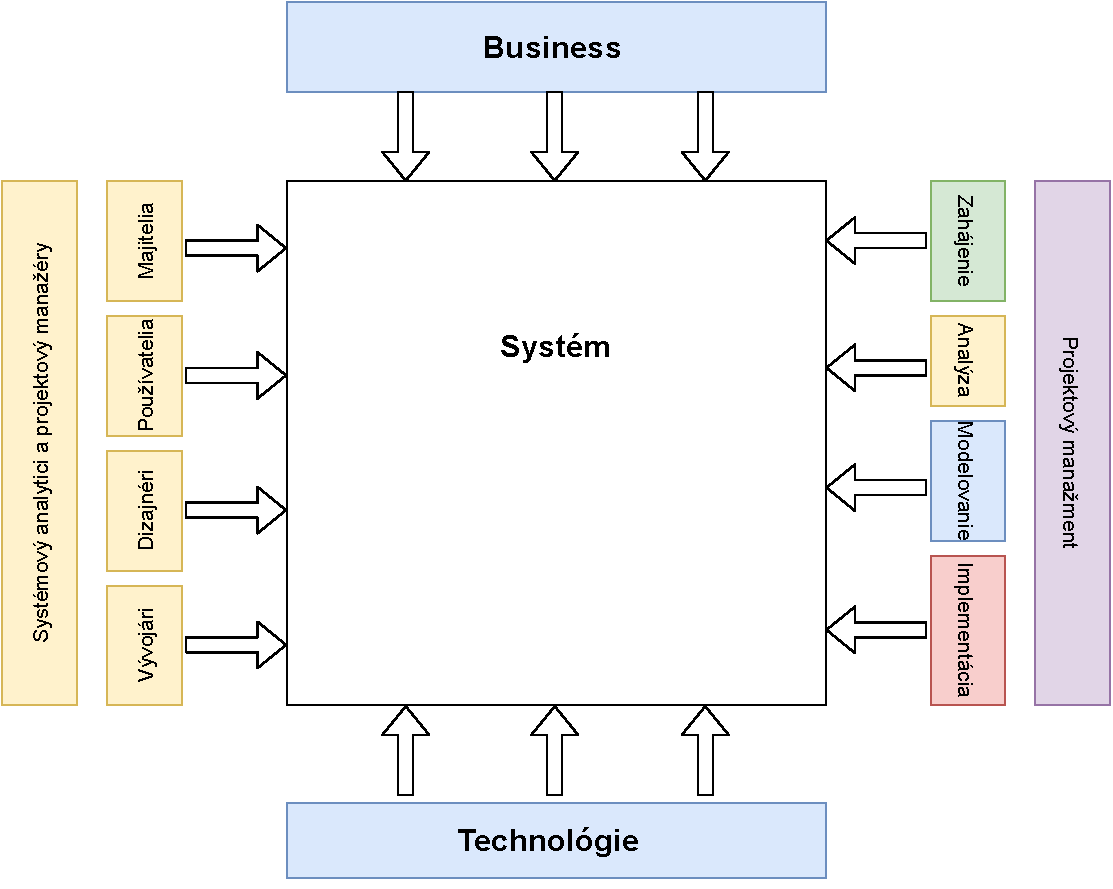
\includegraphics[scale=0.75]{obrazky-figures/TR-system-inputs}
	\caption{Aspekty ovplyvňujúce vývoj systému \cite{whitten2007systems}}
	\label{fig:system-inputs}
\end{figure}

\subsection{Iné factory}
Okrem Účastníkov vývoja majú na systém vplyv ešte aspekty businessu a technológie dostupné v dobe vývoja. Business pokrýva hlavne požiadavky obchodu spojené s legislatívou. Technológie nás obmedzujú pri nedostupnosti tak pokročilých technológií aké by sme potrebovali pre svoj systém alebo naopak nové prielomy v technológii poskytujú príležitosť pozdvihnnúť projekt na vyššiu úroveň.

\subsection{Procces vývoja}
\label{proces_vyvoja}

Je zrejmé že väčšina organizácií bude mať vlastný formálne definovaný proces vývoja softvéru alebo sadu krokov, ktoré podľa ktorých by sa mal systém vyvíjať. Akiste sa budú tieto metodológie od seba diametrálne odlišovať pre jednotlivé organizácie. Avšak, všetky metódy riešenia problému môžeme zavšeobecniť na kroky, ktoré sú spoločné: \\

\begin{enumerate}
	\item \textbf{Identifikovať problém}, akokoľvek jednoducho prvý krok môže znieť opak je pravdou. Zadania sú často nejasné a ciele systému preto nejednoznačné. Rozsah práce môže byť podcenený s čím ide ruka v ruke aj časový plán a rozpočet.
	\item \textbf{Analyzovať a porozumieť problému}. Druhý krok poskytuje projektovému tímu hlbšie porozumenie systému, vyžaduje spoluprácu so zúčastnenou stranou \ref{}.
	\item \textbf{Identifikovať požiadavky a očakávania riešenia}, ktoré kľadú nároky obchodu či funkcionálna stránka vyžadovaná uživateľmi.
	\item \textbf{Identifikovať alternatívne riešenia} a zvoliť najvhodnejšiu cestu. Pri výbere zohráva rolu rozpočet (finančný i časový), predispozície relizačného tímu a uprednostnené cieľe.
	\item \textbf{Navrhnúť zvolené riešenie}, pomocou jednou z metód modelovania systémov.
	\item \textbf{Implementovať zvolené riešenie} za pomoci vymodelovaného návrhu. Náročnosť implementácie je nepriamo úmerná kvalite návrhu.
	\item \textbf{Vyhodnotiť výsledok.} Na záver je nutno objektívne zhodnotiť výsledky v zmysle splnenia cieľov. Pri nesplnení sa môžeme vrátiť ku kroku 1 a 2.
\end{enumerate}
\vspace{1cm}
Na obrázku \ref{fig:system-inputs} je na pravej strane zobrazený pohľad procesu vývoja, ktorý bol kvôli jednoduchosti zredukovaný len na 4 fáze. Táto zjednodušená varianta postačuje na pokrytie problematiky analýzy a modelovania systému. Inizializácia je fáza predchádzajúca analýze a implementácia je niečo, čo prirodzene nadväzuje za úspešným návrhom systému. Jednotlivé kroky zovšeobecneného riešenia problémov do fáz vývoja je v tabuľke \ref{tab:map-steps}. \\

\begin{table}[ht]
	\begin{center}
		\begin{tabular}{| p{6cm} |p{8.5cm}|}
			\hline
			& \\
			\textbf{Zjednodušený vývojový proces} & 
			\textbf{Kroky zovšeobecneného riešenia problémov} \\ [2.5ex] 
			\hline\hline
			\begin{itemize}
				\item[] Zahájenie
			\end{itemize} & 
			\begin{enumerate}
				\item Identifikovať problém
			\end{enumerate} \\ 
			\hline
			\begin{itemize}
				\item[] Analýza systému
			\end{itemize} & 
			\begin{enumerate}
				\setcounter{enumi}{1}
				\item Analyzovať a porozumieť problému
				\item Identifikovať požiadavky a očakávania riešenia
			\end{enumerate} \\
			\hline
			\begin{itemize}
				\item[] Modelovanie systému
			\end{itemize} &  
			\begin{enumerate}
				\setcounter{enumi}{3}
				\item Identifikovať alternatívne riešenia a zvoliť najschodnejšiu cestu
				\item Navrhnúť zvolené riešenie
			\end{enumerate} \\
			\hline
			\begin{itemize}
				\item[] Implementácia systému
			\end{itemize} & 
			\begin{enumerate}
				\setcounter{enumi}{5}
				\item Implementovať zvolené riešenie
				\item Vyhodnotiť výsledok
			\end{enumerate} \\ [1ex] 
			\hline
		\end{tabular}
	\caption{Namapovanie krokov zovšeobecneného postupu do jednotlivých fáz zjednodušeného vývojového procesu.}
	\label{tab:map-steps}
	\end{center}

\end{table}

\section{Analýza systému}
 V sekcii \ref{proces_vyvoja} sme zaradili analýzu systému na svoje miesto v procese vývoja za fázu zahájenia projektu a pred fázu návrhu systému. Z toho vyplýva, že analýza je prerekvizita k úspešnému návrhu systému. Keďže sa v literatúre nestretneme s presne vytíčenou hranicou, kde končí analýza systému a začína návrh systému, v tejto práci bude analýza pokrývať potreby majiteľov a uživateľov systému. Technické a implementačné detaily nebudeme v tejto práci uvažovať ako súčast analýzy. V predchádzajúcej sekcii bola opísaná zúčastnená strana podieľajúca sa na analýze a cieľe analýzy, no samotná otázka "ako analyzovať systém" bola doteraz len nonšalantne opomíjaná. V tejto kapitole budú rozobrané vybrané metodológie a prístupy, ktoré obšírny pojem analýza systému zastrešuje.
 
 \subsection{Prístupy k analýze systému}
Analýza je hlavne o riešení problému, a keďže riešiť problém sa dá viacerími prístupmi, asi nikoho neprekvapí, že aj prístupov k analýze systému bude viac.

\subsubsection{Modelom riadená analýza}
Či sa jedná o štruktúrovanú analýzu, informačné inžinierstvo alebo objektovo-orientovanú analýzu, všetky tri príklady patria do skupiny modelom riadených analýz. Tento prístup používa na vyjadrovanie všetkým zrozumiteľné obrázky na opis problémov, požiadavkov a riešení v systéme. Takou grafickou reprezentáciou môžu byť napríklad vývojové diagramy, štrukturované grafy a iné schémy.

\begin{enumerate}
	\item \textbf{Štruktúrnej analýza}, ako jedna z tradičných foriem analýzy zo 70. rokov používaná do dnes je zameraná na tok dát a analyzuje systém z pohľadu procesov. :TODO: obr dataflow
	\item \textbf{Informačné inžinierstvo} ako ďaľší tradičný prístup narozdiel od sledovania dát v procese, sleduje štruktúru uloženia dát naprieč systémom.
	\item \textbf{Objektovo-orientovaný prístup} sa odlišuje od tradičných prístupov, ktoré sa zámerne snažili oddeliť dáta a procesy. Objektovo-orientovaný prístup zlúčil dáta a procesy do objektov, ktoré majú uložené atribúty objektov (dáta) a metódy objektov, ktoré vykonávajú operácie nad týmito dátami (procesy nad dátami). Objektová orientácia sebou prináša celú sadu nástrojov na modelovanie tzv. jazyk UML (Unified Modeling Language). Jazyku UML bude venovaná celá sekcia :TODO:
\end{enumerate}

\subsubsection{Prototypovanie}
Okrem modelovo orientovanej analýzi môžme skúmať možnosti systému štýlom "Vieme, čo chceme, keď to uvidíme". Tento prístup spočíva vo vytváraní funkčných, ale neúplných prototypov výsledného systému, ktoré sa postupnou iteráciou dostanú k požadovanému systému. Slovom neúplných myslíme prototyp bez 
 
  


\section{Návrh systému}


\section{UML}
\begin{enumerate}
	\item Diagram Použitia
	\item Diagram Aktivít
	\item Diagram Tried znázorňuje systémovú objektovú štruktúru. Ukazuje triedy objektov, ktoré v systéme figurujú ako aj ich väzby medzi sebou.
\end{enumerate}

\section{Proces vývoja software}
Systémy a produkty v 50. rokoch boli primárne hardvérového charakteru. Logické a matematické výpočetné procesy boli implementované pomocou elektromechanických zariadení. V 60. rokoch už integrované obvody umožnili vývojárom zvýšiť spolahlivosť a presnosť výpočtovej techniky do istej miery aj zásahom softwéru. V tejto dobe však chyby alebo zmeny návrhu boli drahé a časovo náročné.
S Príchodom mikroprocesorovej technológie, začatkom 70. rokov, sa software stal schodnou alternatívou pre integrované obvody. Schopnosti systému, ktoré museli byť inak implementované pomocou harvéru zrazu boli implementovateľné omnoho jednoduchšie a rýchlejšie softwarom. Výsledokom bola evolúcia v návrhu systému, ktoré začali modelovať flexibilné a rekonfigurovateľné systémy.\cite{wasson2006system} To umožnilo vývojárom vytvárať špecifické aplikácie len jednoduchým prispôsobením softwaru.
Prechod k softwérovým systémom nastal ešte pred vznikom metód na produkovanie softwaru. Keď sa aplikácie stávali robustnejšími a komplexnejšími zvyšoval sa aj risk a pribúdali problémové oblasti. Dodržanie technických očakávaní, rozpočtu, a času odovzdania boli hlavné problémy. Vznikla potreba pre opakovanie a predvídateľnosť úspešných vývojových procesov. Začali vznikať opakovateľné metodológie procesu vývoja. software.
\subsection{iteratívny}
Iteratívne procesy akceptujú možnosť zmien a opakujú do istej miery fáze požiadavok, designu a implementácie. Jedným z iteratívnych procesov je Rational Unified Process (RUP)
\subsection{štrukturovaný}
Štrukturované modely striktne oddeľujú jednotlivé etapy vývoja, to ich robí nepraktickými pre dnešnú turbulentnú dobu, kde sa špecifikácie systému menia aj za behu vývoja software. Predstaviteľom tohto prístupu je napríklad model Vodopád (Waterfall). Vznikol ako Jeden z prvých pokusov charakterizovať softwarový vývoj ako model. Ilustrácia je na Obr. \ref{fig:waterfall_model}.

\begin{figure}[H]
	\label{fig:waterfall_model}
	\centering
	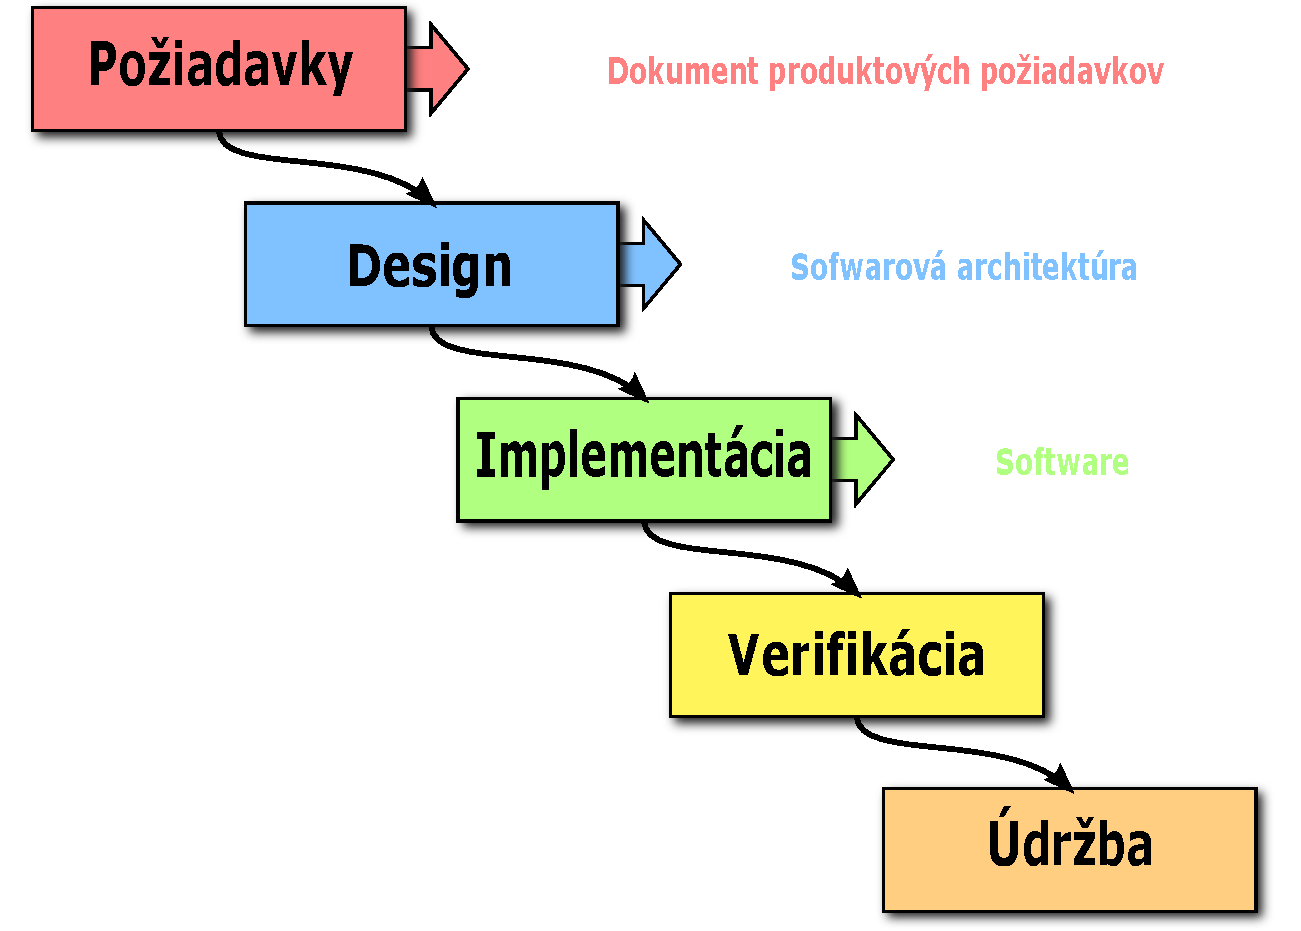
\includegraphics[scale=0.5]{obrazky-figures/TR-waterfall-model}
	\caption{Vodopádový model}
\end{figure}

Vo \textbf{vodopád}ovom modely sú vývojové etapy vykonávané sekvenčne s minimálnym prekrytím a bez iterácií medzi etapamy. Šípky nevedú naspäť do predchádzajúcich etáp. Uživateľské potreby sú stanovené. Požiadavky sa nemenia. Celý systém je navrhnutý, implementovaný a otestovaný pre konečné odovzdanie.


\subsection{inkrementálny}

\subsection{Agilný}
Tento prístup sa vyznačuje flexibilitou. Funguje na princípe extrémne krátkych iterácií. V tomto procese máme fungujúci systém, ktorý neustále rozširujeme. 

\section{Tvorba scenárov} 

Scenár môže byť chápaný celou radou interpretácií, niektoré z nich sú uplatniteľné v systémovom inžinierstve. Scenár môže byť sekvencia aktivít alebo rozhodovací strom viacerých takýchto sekvencií. Vetvy rozhodovacieho stromu reprezentujú alternatívy, či rôzne možnosti chovania systému. Zložitosť scenára je závislá na rozvetvení rozhodovacieho stromu. Scenár môže byť konkrétny či abstraktný \cite{scenarios}. V tejto práci sa budeme zaoberať výlučne konkrétnym scenárom systému, abstrakcia sa zo scenáru odstráni doménovým modelovaním. Viac o tejto probelmatike v sekcii \ref{sec:TR-domain-modeling}.

Scenár môže byť chápaný celou radou interpretácií, niektoré z nich sú uplatniteľné v systémovom inžinierstve. Scenár môže byť sekvencia aktivít alebo rozhodovací strom viacerých takýchto sekvencií. Vetvy rozhodovacieho stromu reprezentujú alternatívy, či rôzne možnosti chovania systému. Zložitosť scenára je závislá na rozvetvení rozhodovacieho stromu. Scenár môže byť konkrétny či abstraktný \cite{scenarios}. V tejto práci sa budeme zaoberať výlučne konkrétnym scenárom systému, ako súčasť požiadavkov systému definovaných pri analýze systému. Takýto konkrétny scenár bude pohľad na systém zachytávajúci prípad užitia.


\chapter{Petriho Siete}
V tejto kapitole je popísaná obecná Petriho sieť a formalizmy, ktoré vedú k jej transformácii na varianty Petriho sietí s potrebnými vlastnosťmi pre automatické generovanie sekvenčných diagramov.

\section{Obecná definícia}
Ako východziu Petriho sieť pre ďalšie varianty a rozšírania použijeme sieť definovanú v literatúre ako PT-sieť (Place/Transition Net), [Pet81, Rei85], je zobecnením jednoduchšieho modelu CE-sietí (Condition-Event Net).

\begin{note}
	CE-sieť narozdiel od PT zobecnenia umožňuje do miest ukladať len jednu značku, miesta v tejto sieti nadobúdajú len booleovských hodnôt. Prechody CE-sietí sú provediteľné len za podmienky, že sú vstupné podmienky pravdivé a výstupné nepravdivé (hodnota 0 vo všetkých výstupných miestach). Obsah práce nevyžaduje uchopenie teórie až do hĺbky CE-sietí, preto vychádzame z tohto jej zobecnenia. 
\end{note}

\begin{defn} Petriho sieť je štvorica $N = (P_N, T_N, PI_N, TI_N)$, kde \begin{enumerate}
	\item $P_N$ je konečná množina miest
	\item $T_N$ je konečná množina prechodov, $P_N \cap T_N$
	\item $PI_N : P_N \longrightarrow  \mathbb{N}$ je inicializačná funkcia
	\item $TI_N$ je popis prechodov (transition inscription function) definovaných tak,\\
	\quad že $\forall t \in T_N : TI_N(t) = (PRECOND_t^N, POSTCOND_t^N)$,\\
	kde
	\begin{enumerate}
		\item $PRECOND_t^N : P_N \longrightarrow \mathbb{N}$ sú vstupné podmienky (vstupy) prechodu
		\item $POSTCOND_t^N : P_N \longrightarrow \mathbb{N}$ sú výstupné podmienky (výstupy) prechodu
	\end{enumerate}
\end{enumerate} \end{defn}

Pre potreby grafickej reprezentácie Petriho siete definujeme množinu hrán.

\begin{defn}
	Množina hrán Petriho siete $A_N$
	$$ A_N \subseteq (P_N \times T_N) \cup (T_N \times P_N)$$
	pričom platí, že
	$$ \forall (p,t) \in (P_N \times T_N) [(p,t) \in A_N \Longleftrightarrow PRECOND_t^N(p) > 0 ]$$
	$$ \forall (t,p) \in (T_N \times P_N) [(t,p) \in A_N \Longleftrightarrow POSTCOND_t^N(p) > 0 ]$$
\end{defn}

\begin{defn}
	Ohodnotenie hrán je funkcia $W_N : A_N \longrightarrow \mathbb{N}$ pre ktorú platí
	$$ \forall (p,t) \in A_N \cap (P_N \times T_N) [W_N(p,t) = PRECOND_t^N(p) ]$$
	$$ \forall (t,p) \in A_N \cap (T_N \times P_N) [W_N(t,p) =  POSTCOND_t^N(p)]$$
	ak $(p,t) \in A_N \cap (P_N \times T_N)$ vravíme, že $p$ je \textbf{vstupné miesto} a $(p,t)$ je \textbf{vstupná hrana} prechodu $t$. ak $(t,p) \in A_N \cap (T_N \times P_N)$ vravíme, že $p$ je \textbf{výstupné miesto} a $(t,p)$ je \textbf{výstupná hrana} prechodu $t$.
\end{defn}

Stav systému Petriho siete je určený rozmiestnením značiek v miestach.

\begin{defn}
	\textbf{Značenie siete} $N$ je funkcia $M : P_N \longrightarrow \mathbb{N}$. Funkcia $M_0 = PI_N$ je počiatočné značenie siete $N$.
	
\end{defn}

	Dynamika Petriho sietí spočíva vo vykonávaní prechodov. Ich provediteľnosť závisí na značeniu siete a naopak. Tieto závislosti popisujú evolučné pravidlá.
	
\begin{defn}
	\textbf{Evolučné pravidlá} \\\\ Majme sieť $N$ a jej značenie $M$.
	\begin{enumerate}
		\item Prechod $t \in T_N$ je \textbf{provediteľný} v značení $M$ práve vtedy, keď
		$$ \forall p \in P_N [PRECOND_t^N(p) \leq M(p) ]$$
		\item Ak prechod $t \in T_N$ je provediteľný v značeniu $M$, môže byť \textbf{prevedený}, čo zmení značenie $M$ na $M'$, definované ako:
		$$\forall p \in P_N [M'(p)=M(p) - PRECOND_t^N(p) + POSTCOND_t^N(p) ]$$ 
	\end{enumerate}
\end{defn}  



Stav systému, popsaného množinou stavových strojov, je určený množinou stavov jednotlivých strojov. Stav (stavová premená) systému je distribuovaný do množiny parciálních stavov systému. Prechody sa vykonávajú v jednotlivých strojoch je však potreba synchronizovat

Parciálne stavy systému sú modelované miestamy a vzormi mo¾ných událostí jsou denovány
pøechody. Místo se v grafu Petriho sítì vyjadøuje jako 
 a pøechod jako . Okam¾itý stav
systému je denován umístìním znaèek (tokens) v místech, co¾ v grafu Petriho siete vyjadrujeme
teèkami v místech. Prítomnost značky v místì modeluje skuteènost, ¾e daný aspekt stavu (parci
ální stav) je momentálnì aktuální, resp. podmínka je splnìna. Ka¾dý pøechod má denována
vstupní a výstupní místa, co¾ je v grafu Petriho sítì vyjádøeno orientovanými hranami mezi
místy a pøechody: 
! a !
. Tím je deklarováno, které aspekty stavu systému podmiòují
výskyt odpovídající události (provedení pøechodu), a které aspekty stavu jsou výskytem této

\subsection{Paralelizmus v Petriho sietiach}

Paralelizmus môže byť prenesený do Petriho sietí viacerými spôsobmi.
\begin{enumerate}
	\item Presdtavme si príklad dvoch triviálnych konkurenčných procesov. Každý môže byť reprezentovaný Petriho sieťov, nech $p \in P_N$ a nech miesto $p$ je zdielané oboma procesmi. 
	
	\begin{figure}[H]
		\label{fig:example-proc}
		\centering
		\includegraphics[scale=0.5]{obrazky-figures/PN-process1}
		\caption{Ukážkový proces}
	\end{figure}
	
	Jednoducho \textbf{zložením} oboch \textbf{sietí} dostaneme jednu. Táto zložená siet na Obr. \ref{fig:parallel-proc} inicializuje dve značky, pre každý proces jednu, tákáto inicializácia vo výpočetných systémoch možná nie je, preto je tento spôsob pramálo využiteľný.
	
	\begin{figure}[H]
		\label{fig:parallel-proc}
		\centering
		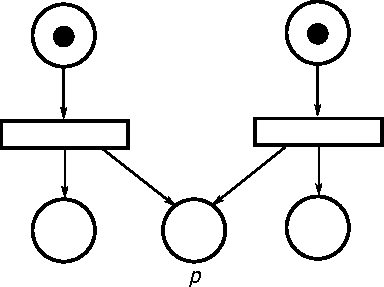
\includegraphics[scale=0.5]{obrazky-figures/PN-parallel2}
		\caption{Ukážka zloženia dvoch sietí. V praxi neužitočné.}
	\end{figure}

	\item Ďaľší prístup je zvážiť ako sa k paralelizmu pristupuje vo výpočetných systémoch. Niekoľko návrhov je schodných. Jeden z najjednoduchších zahŕňa operácie \textbf{FORK} a \textbf{JOIN}. Operácie boli pôvodne navrhnuté Jackom Dennisom a Earlom Van Hornom v roku 1966. Ich prevedenie do Petriho siete je nasledovné: 
	
	\begin{figure}[H]
		\centering
		\begin{minipage}{.4\textwidth}
			\label{fig:fork}
			\centering
			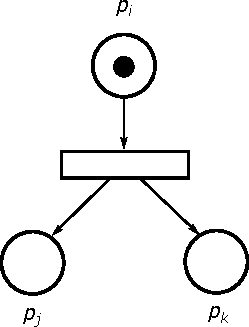
\includegraphics[scale=0.5]{obrazky-figures/PN-fork}
			\caption{Operácia FORK vykonaná v mieste $p_i$ vytvorí proces v miestach $p_j$ a $p_i$.}
		\end{minipage}
	\begin{minipage}{.05\textheight} %spacer
		\quad
	\end{minipage}
		\begin{minipage}{.4\textwidth}
			\label{fig:join}
			\centering
			\includegraphics[scale=0.5]{obrazky-figures/PN-join}
			\caption{Operácia JOIN vykonaná za koncovými miestami procesov $p_j$ a $p_k$ ich spojí a pokračuje v mieste $p_i$.}
		\end{minipage}
	\end{figure}
	
	\item Iný návrh zavedenia paralelizmu je riadiaca štruktúra \textbf{parbegin} a \textbf{parend} [Djikstra 1968]. Koncept navrhnutý Djikstrom má všeobecnú formu $parbegin$ $S_1; S_2;$\dots$S_n$ $parend$, kde $S_i$ predstavuje výraz. Význam $parbegin | parend$ štruktúry je vykonať každý výraz $S_1; S_2;$\dots$S_n$ paralelne. Prevedenie v Petriho sieti je na Obr. \ref{fig:parbegin}.
	
	\begin{figure}[H]
		\centering
		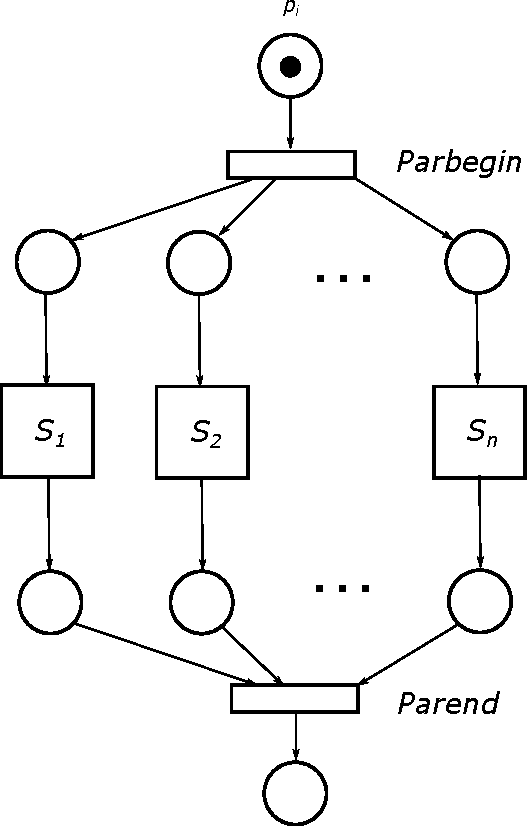
\includegraphics[scale=0.5]{obrazky-figures/PN-parbegin}
		\caption{Riadiaca štruktúra \emph{parbegin} a \emph{parend} v Petriho sieti}
		\label{fig:parbegin}
	\end{figure}
	
	
\end{enumerate} 

\subsection{Čas v Petriho sietiach}

\subsection{Varianty petriho Sietí}
Petriho siete sú koncipované ako plošný (neštrukturovaný) model, kde hierarchický aspekt modelovaného systému nie je nijak vyjadrený. Varianty spomenuté v tejto sekcii sa budú zaoberať rozšírením výpočetnej a modelovacej sily nezbytnej pre prekonanie problému spojeného s plošným statickým modelom. \\\\
\subsubsection{Inhibítory}
Inhibítory umožňujú testovať počet značiek v mieste a tým dávajú Petriho sietiam výpočetnú silu Turingového stroja a sú teda schopné počítať všetky vyčísliteľné funkcie. Takouto sieťou je možné špecifikovat ľubovoľný algoritmus.
\subsubsection{Vysokoúrovňové Petriho siete}
Napriek tomu, že sú siete s inhibítormi schopné vyjadriť akýkoľvek algoritmus, modelovanie čo i len prostého vyhodnocovania aritmetických výrazov je príliš zložité a neintuitívne. Dôvodom sú prostriedky, ktoré zahŕňajú len odjímanie značiek zo vstupných miest a pridávanie značiek do miest výstupných. HL-Siete riešia tento problém zavedením konceptu hranových výrazov, prechodovej stráže a prechodovej akcie.

K tomu, aby sme mohli vysvetliť základné koncepty HL-sítí, potrebujeme pomocný pojem multimnožina a operáciie s multimnožinami.
\begin{defn}
	Majme ľubovolnú neprázdnu množinu $E$. Multimnožina nad množinou $E$ je funkcia. $x : E \longrightarrow \mathbb{N}$. Hodnota $x(e)$ je počet výskytov (koeficient) prvku $e$ v multimnožine $x$. Multimnožinu zapisujeme ako formálnu sumu 
	$$ \sum_{e \in E} x(e)'e $$
	Množinu všetkých multimnožín nad $E$ označíme $E^{MS}$. Pre multimnožiny $x$, $y$ nad $E$ a prirodzené číslo $n$ definujeme:
	
	\begin{enumerate}
		\item sčítanie: $$x + y = \sum_{e \in E} (x(e) + y (e))`e$$
		\item skalárne násobenie: $$n`x = \sum_{e \in E}^{} (n x(e))`e$$
		\item porovnanie:
		$$ x \neq y = \exists e \in E [x(e) \neq y(e) ]$$
		$$ x \leq y = \forall e \in E [x(e) \leq y(e) ]$$
		\item odčítanie: $$x - y = \sum_{e \in E} (x(e) - y (e))`e$$
		\item veľkosť: $$|x| = \sum_{e \in E} x(e)$$
	\end{enumerate}
\end{defn}

\begin{exmpl}
	názorne zápis $2`A + 3`B$ predstavuje multimnožinu s troma výskytmi prvku $a$ a štyrmi výskytmi prvku $b$.
\end{exmpl}

\begin{note}
	Koeficient 1 obvykle vynechávame, tj. napríklad zápis $c$ predstavuje rovnakú multimnožinu ako zápis $1`c$.
\end{note}

Takúto Multimnožinu môžeme konceptom \textbf{hranových výrazov} priradiť k hranám vstupným ako aj výstupným. Názorná ukážka je na Obr. \ref{fig:edge-expr}.

\begin{figure}[H]
	\centering
	\begin{subfigure}[t]{0.4\textwidth}
		\centering
		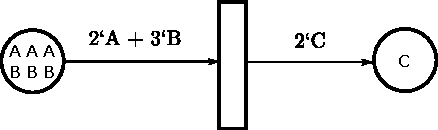
\includegraphics[scale=0.75]{obrazky-figures/PN-edge-expr}
		\caption{Stav pred uskutočnením prechodu}
	\end{subfigure}
	\begin{subfigure}[t]{0.4\textwidth}
		\centering
		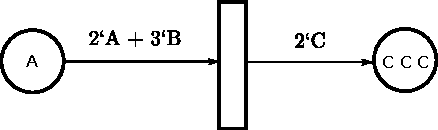
\includegraphics[scale=0.75]{obrazky-figures/PN-edge-exprR}
		\caption{Stav po uskutočnením prechodu}
	\end{subfigure}
	\caption{Hranové výrazy na vstupnej aj výstupnej hrane.}
	\label{fig:edge-expr}
\end{figure}
každému prechodu je možno priradiť \textbf{stráž prechodu}, booleovský výraz, ktorý musí byť splnený pre uskutočnenie prechodu. Je možné určité naviazanie
premenných vo výrazoch na vstupných hranách a rovnako v stráži prechodu. Príklad strážneho výrazu \uv{$x > y$} aj s naväzovaním premenných je na Obr. \ref{fig:guard}.

Pre sugestívnejší zápis dovoluje k stráži prechodu pridať \textbf{akciu prechodu}, odlišujúcu výpočty, ktoré se realizujú pri vykonávaní prechodu, od tých, ktoré se realizujú pri zisťovaní uskutočniteľnosti prechodu.

\begin{figure}[H]
	\centering
	\includegraphics[scale=0.75]{obrazky-figures/PN-guard}
	\caption{Príklad stráže prechodu a akcie prechodu}
	\label{fig:guard}
\end{figure}

\subsubsection{Hierarchické Petriho siete}





\section{PNTalk}

V predošlej kapitole sme sa dozvedeli akú variantu Petriho sietí budeme potrebovať, teraz je na čase predstaviť praktickú implementáciu formalizmu objektovo orientovaných petriho sietí.
\section{Trieda a dedičnosť}

\section{Siete}

\subsection{Objektová sieť}

\subsection{Sieť metód}

\subsection{Sieť konstruktoru}

\subsection{Synchrónny port}

\section{Prechod}

\subsection{Podmienky prechodu}

\subsection{Akcia}

\subsection{Stráž}

\section{PNTalk}

TODO

\chapter{Sekvenčné Diagramy}

Jednou zo štyroch základných modelačných techník UML (Unified Modeling Language) užívanou hojne pri navrhovaní programových systémov je Sekvenčný diagram. Sekvenčný diagram je najbežnejší z kategórie diagramov interakcií a zobrazuje objekty, ktoré sa účastnia v prípade užitia a taktiež zobrazuje správy, ktoré si tieto objekty vymieňajú počas časového intervalu. Diagram je dvojdimenzionálny. Účastníci sú zoradený na horizontálnej ose a časový priebeh je vyjadrený na vertikálnej, kde čas plynie zhora nadol. Ich nespornou výhodou je zobrazovanie aktivity toku správ v časovej postupnosti, to je nápomocné pre porozumenie real-time systémom a komplexným prípadom užitia.

\section{Scenáre}

Sekvenčné diagramy môžu byť generické, zobrazujúce všetky možné scenáre pre definovaný prípad užitia. Častejšie sa však stretneme s vypracovaním diagramov pre jednotlivé scenáre v prípade užitia samostatne.

\section{Komunikácia v sekvenčných diagramoch}

Komunikačný mechanizmus prítomný v sekvenčných diagramoch je, že 
aktivní entity komunikujú priamo, zasielaním správ. 
\begin{note}
	Tu nachádzame konflikt s PT-sieťou v ktorej aktívne entity komunikujú nepriamo, prostredníctvom zdieľaných pasívnych objektov, miestami siete. Mechanizmy sa dajú previesť z jedného na druhý, čo opisuje sekcia :TODO
\end{note}
Sémantika správ je stopa jednoduchej dvojice \lstinline{<sendEvent, RecieveEvent>}, kde \lstinline{sendEvent} je udalosť odoslania správy a \lstinline{recieveEvent} udalosť jej prijatia. Pri absencii jednej udalosti hovoríme o neúplnej správe.

\begin{defn}
	\textbf{Stratená správa} je neúplná správa, pri ktorej je známy výskyt udalosti odoslania správy \lstinline{sendEvent}, ale nie je zaznamenaná udalosť prijatia správy \lstinline{recieveEvent} 
	Typická interpretácia je, že destinácia príjemcu správy je mimo popisovaného rámca. Sémantika je potom zjednodušená na tvar 
	\lstinline{<sendEvent>}.
	Anotácia je šípka vedená od odosielatela zakončená malou bodkou.
\end{defn}

\begin{figure}[H]
	\centering
	\begin{subfigure}[t]{0.4\textwidth}
		\centering
		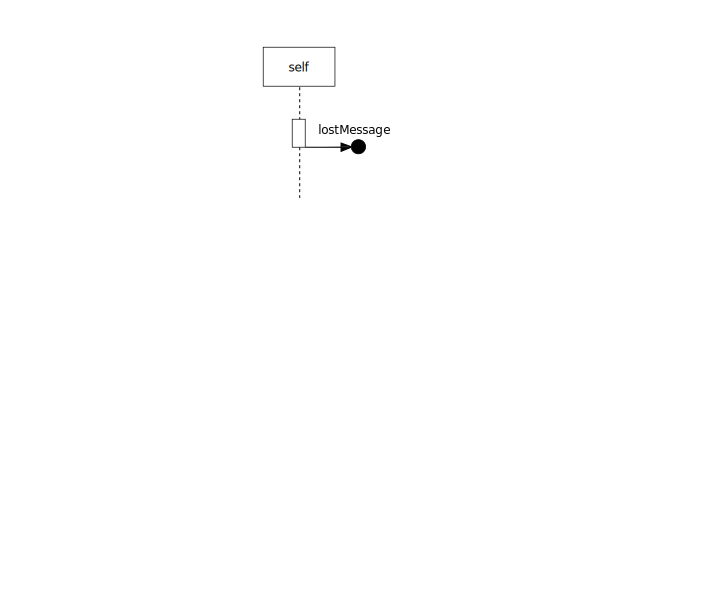
\includegraphics[scale=0.75]{obrazky-figures/SD-lost-ex}
		\caption{Stav pred uskutočnením prechodu}
	\end{subfigure}
	\begin{subfigure}[t]{0.4\textwidth}
		\centering
		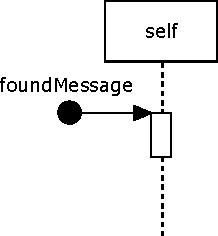
\includegraphics[scale=0.75]{obrazky-figures/SD-found-ex}
		\caption{Stav po uskutočnením prechodu}
	\end{subfigure}
	\caption{Nekompletné správy}
	\label{fig:uncomplete-mes}
\end{figure}

Kompletná správa je v diagrame reprezentovaná orientovanou horizontálnou šípkou smerujúcou od aktívneho objektu odosielateľa k čiare života príjemcu správy. \\\\
V Sekvenčných diagramoch rozlišujeme tri typy správ:

\begin{enumerate}
	\item \textbf{Synchrónna správa} medzi objektami indikuje  sémantiku \emph{wait}, kedy  odosielateľ správy čaká kým je správa spracovaná a pokračuje až po obdržaní odpovede. Správa typicky predstavuje volanie metódy.
	\item \textbf{Asynchrónna správa} používa asynchrónny prístup, pri ktorom nedochádza k žiadnemu blokovaniu objektu odosielateľa. Asynchrónna správa medzi objektami indikuje \emph{no-wait} sémantiku a objekt pokračuje bez toho, aby čakal na odpoveď. Toto dovoľuje paralélne procesy.
	\item \textbf{Odpoveď} predstavuje spätnú správu po synchrónnej správe. Nemôže vzniknúť samostatne.
\end{enumerate}

\begin{figure}[H]
	\centering
	\begin{subfigure}[t]{.3\textwidth}
		\centering
		
\includegraphics{obrazky-figures/SD-sync}
		\caption{Synchrónna správa}
	\end{subfigure}
	\begin{subfigure}[t]{.3\textwidth}
		\centering
		
\includegraphics{obrazky-figures/SD-async}
		\caption{Asynchrónna správa}
	\end{subfigure}
\begin{subfigure}[t]{.3\textwidth}
	\centering
	
\includegraphics{obrazky-figures/SD-reply}
	\caption{Odpoveď}
\end{subfigure}
	\caption{Reprezentácie troch typov správ}
	\label{fig:arrows}
\end{figure}

\section{Účastníci komunikácie}
Participanti komunikácie skrz správy popísané vyššie sú aktívne objekty, ktoré v sekvenčných diagramoch reprezentujeme čiarou života(\emph{lifeline}).

\begin{defn}
	Pri definícii \textbf{čiary života} začneme netradične notáciou, je zobrazená vertikálnou čiara (môže byť čiarkovaná) predstavujúcu čas života aktívneho objektu. Na jej počiatku sa nachádza hlavička, obdĺžnik obsahujúci \textbf{identifikačnú informáciu} vo formáte: \\
	%\begin{lstlisting}
%<lifelineident> ::= ([<connectable-element-name>[‘[‘ <selector> %‘]’]]
%		[: <connectable-element-type>] [<decomposition>]) | ‘self’
%<selector> ::= <expression>
%<decomposition> ::= ‘ref’ <interactionident> [‘strict’]
%	\end{lstlisting} \vspace{.5cm}
	
	kde \lstinline{<connectable-element-name>} referuje meno typu pripojeného elementu reprezentovaného množinou dodatočných interných datových štruktúr. Napriek tomu, že to zápis dovoľuje \lstinline{<lifelineident>} nemôže byť prázdny.
	
	Ak je identifikátor 'self' čiara života reprezentuje objekt klasifikátoru interakcie, ktorá sama vlastní čiaru života.
	
	
\end{defn} 

\section{Stavebné Elementy sekvenčných Diagramov}

V nasledujúcej sekcii je popísaná syntax a sémantika sekvenčných diagramov.

\subsection{Actor:TODO preklad}

\subsection{objekt}

\subsection{lifeline:TODO preklad čiara života? :D}

\subsection{focus of control:TODO preklad}

\section{Distribuované systémy}

Distribuované systémy majú veľa rozdielnych aspektov, ktoré sa ťažko zachytávajú v jednej difinícii. Je omnoho jednoduchšie hovoriť o distribuovaných systémoch špecifikovaním charakteristík, symptómmi, či média distribúcie. \cite{} V tejto práci budeme mať pod pojmom distribuovaný systém uvažovať systém distribuovaný na počítačovej sieti. \\

Distribúcia prichádza ruka v ruke s vednými disciplínami ako tolerácia chýb, real-time systémy, bezpečnosť a systémový manažment

\subsection{Vymedzenie pojmu distribuovaný systém}

Pred definovaním distribuovaného systému, je vhodné vyjasniť rozdiel s často zameňovaným pojmom počítačových sietí.

\begin{displayquote}
	``Počítačová sieť nie je distribuovaný systém.''
\end{displayquote}

\textbf{Počítačová sieť} je infraštruktúra slúžiaca niekoľkým počítačom  pripojeným k sieti cez komunikačné prepojenie realizované rôznymi médiami a topológiami, a používajú zavedný komunikačný protokol.
Zatiaľ čo \textbf{Distribuovaný systém} je systém pozostávajúci z niekoľkých počítačov, ktoré komunikujú cez počítačovú sieť, hosťujú procesy, ktoré využívajú distribučné protokoly, ktoré zabezpečujú koherentné vykonanie distribuovaných aktivít. \\

\begin{exmpl}
	Vezmime si taký Internet, je to rozsiahla počítačová sieť, vlastne najpodstatnejšia sieť dnes. Používa TCP/IP ako komunikačný protokol.
	Napriek tomu, že tradične poskytuje zopár aplikačných služieb ako e-mail a telnet, nie je to distribuovaný systém. \\
	
	To samozrejme nebráni distribuovaným systémom byť postavených na internete alebo používania internetových technológií, ako distribuované súborové systémy a databázové systémy.
	Jeden z najpodstatnejšįch rozdieľov je, že v prípade distribuovaných systémov procesy zdieľajú spoločný stav a spolupracujú na dosiahnutí spoločného cieľu. Narozdiel od procesov v tomto príklade, ktoré nemusia spolupracovať, len si napríklad vymieňať správy (ako e-mail) bez spoločného cieľu.
\end{exmpl}

\subsection{Porovnanie s Centralizovanými systémami}

V Tabuľke \ref{Tab:central_vs_distr} sú zaznamenané vlastnosti v porovanní s centrálnym systémom ako protipólom k distribuovanému systému. Poznanie rozdieľov, výhod a nevýhod oboch systémov je kľúčové pri návrhu systému. Na základe týchto informácií sa možno ľahšie rozhodnúť, ktorú variantu zvoliť.

\begin{table} [ht]
\begin{center}
	\begin{tabular}{| c | c |} 
		\hline
		Centralizované systémy & Distribuované systémy \\ [0.5ex] 
		\hline\hline
		Dostupnosť & Geografický rámec \\ 
		Homogenita & Heterogenita \\
		Spravovateľnosť & Modularita \\
		 & Škálovateľnosť \\
		 Konzistencia & Zdieľanie \\
		 & Pozvoľná degradácia \\
		 Bezpečnosť & Bezpečnosť \\
		 & Finančný faktor \\ [1ex] 
		\hline
	\end{tabular}
\end{center}
\caption{Porovnanie centralizovaných a distribuovaných systémov}
\label{Tab:central_vs_distr}
\end{table}

Centralizované systémy prirodzene prichádzajú s ľahkou \textbf{dostupnosťou} zdrojov a informácii systému, keďže sú lokálne dostupné. Na druhú stranu Distribuované systémy majú potencionálne \textbf{široký geografický rámec}, preto prístup k zdrojom je niekedy možný len cez vzdialené procedurálne volania.

 \textbf{Homogenita} technológií a procedúr je charakteristická pre centralizované systémy, čím sa myslí jeden operačný systém pre celý systém, ťažké odklonenie sa od používaných technológií systému (programovací jazyk, aplikační rámec). Kdežto u distribuovaných systémov je podporovaná \textbf{heterogenita}, ktorá dovoľuje mať pre každú komponentu odlišné prostredie. Homogenita zjednodušuje správu centrálnych systémov. Heterogenita činí distribuovaný systém inkrementálne rozšíriteľný, ikeď centralizované systémy môžu s dodržaním homogenity dosiahnuť rovnaké rozmery. Skutočná výhoda je až pri \textbf{škálovateľnosti}, kedy centralizované systémy môžu škálovať len \textbf{vertikálne}, to jest zlepšovať výkon nahradzovaním hardvéru za výkonnejší na svojej jednej centrálnej inštancii. Takéto škálovanie je obmedzené technológiou, hardvér sa nedá zlepšovať do nekonečna. Pri distribuovanom systéme máme možnosť škálovať \textbf{horizontálne}, obsluhovať dosiahnutie spoločného cieľu na viacerých inštanciách zároveň. Rozdieľ medzi vertikálnym a horizontálnym škálovaním je graficky znázornený na obrázku \ref{fig:scaling}. 

\begin{figure}[H]
	\centering
	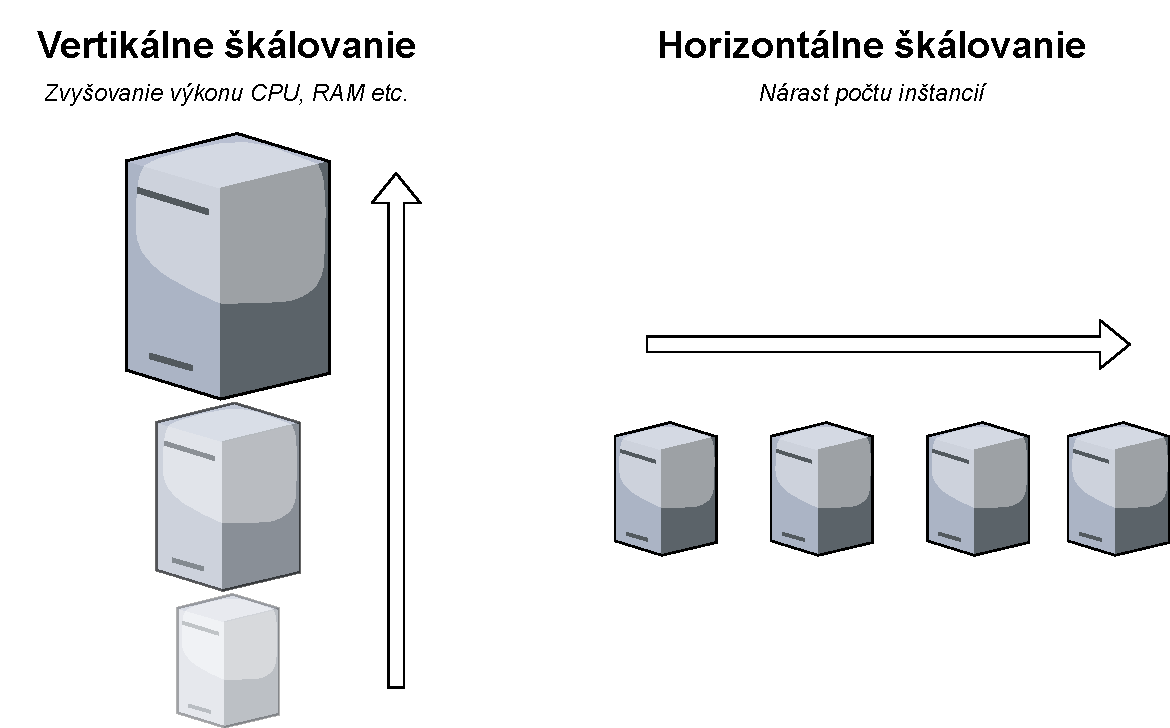
\includegraphics[scale=0.6]{obrazky-figures/TR-scaling}
	\caption{Vertikálne a horizontálne škálovanie}
	\label{fig:scaling}
\end{figure}

\textbf{Konzistenciu} ľahšie dosiahneme u centralizovaných systémov, u distribuovaných je obtiažnejšie zachytiť globálny stav naprieč širokým globálnym rámcom všetkých komponent. \textbf{Pozvoľná degradácia} je vlastnosť systému, ktorý beží kontinuálne spôsobom opatrujúcim možnosť zlyhania komponenty spôsobom, ktorý predíde zlyhaniu celého systému. Tu možno pozorovať silu distribučného systému, kedy pri zlyhaní menšej časti je systém stále dostupný vďaka vysporiadavaniu sa s chybami. Navyše je nepravdepodobné zlyhanie všetkých komponent v rovnaký čas kvôli geografickej separácii jednotlivých komponent.

\textbf{Bezpečnosť} sa dosahuje ľahšie u izolovaného systému s fyzickým prístupom. To nie je možné u distribuovaného systému, avšak vysoká miera bezpečnosti sa dá zaistiť zameraním sa na redukovanie negatívneho efektu vniknutia do systému, než redukovaním hrozieb vzniku neoprávneného vniknutia.

Shrnutím vidíme, že výhody značne prevyšujú ak sa správne rozhodneme, kedy je potreba systém distribuovať.

\subsection{Kedy distribuovať}


Keď nepotrebujeme distribuovaný systém, tak zásadne nedistribujeme. Zbytočne by sme si tým skomplikovali život. Odpoveď pozostáva z troch esenciálnych príčin prečo distribuovať

\begin{enumerate}
	\item Keď má riešený problém decentralizovanú podstatu \\
	\begin{exmpl}
		Zriadujeme systém používajúci konkurenntné procesy na zdrojoch vzdialených pobočiek.
	\end{exmpl}
	\item Keď techniky distribúcie sú vhodnou súčasťou riešenia \\
	\begin{exmpl}
		Systém banky, ktorá potrbuje zálohovať a synchronizovať dáta v dvoch geograficky odľahlých miestach
	\end{exmpl}
	\item Keď problém predpokladá časté zmeny a evolúciu funkcionality, či presunu geografickej polohy. \\
	\begin{exmpl}
		Systém prepožičiavania výpočetných zdrojov medzi vzdialenými uživateľmi.
	\end{exmpl}
\end{enumerate}

\section{Vývojové prostredie}
	Táto kapitola sa zaoberá rozborom vývojových prostredí a ich dekompozíciou na jednotlivé editory a grafické nástroje prítomné v úspešných vývojových prostrediach. \\
	
	Ich význam spočíva v uľahčení práce programátora, zefektívnením kódovania a rýchelho detekovania problémov. Prostredie vedie programátora cez proces editovania, kompilácii či interpretovania kódu a odľaďovania(debugging).
	
	\subsection{Projektový pohľad}
	Predtým než sa pustíme do editovania kódu, musí vývojové prostredie naviazať spojenie s operačným systémom a jeho súborovým systémom. Pri otvorení projektu sken koreňového adresára nahrá do vývojového prostredia kópie súborov a zobrazí ich graficky v projektovom pohľade. Väčšinou je na grafickom uživateľskom rozhraní zobrazovaný pomocou hierarchického stromu, kde listy sú súbory projektu a uzly sú adresáre.
	
	\begin{figure}[H]
		\label{fig:ui-project-pane}
		\centering
		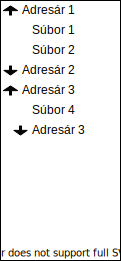
\includegraphics[scale=0.75]{obrazky-figures/UI-project-pane}
		\caption{Ukážka projektového pohľadu s využitím stromovej štruktúry}
	\end{figure}
	
	
	\subsection{Editor zdrojového kódu}
	\label{sec:TR-code-editor}
	Neoddeliteľnou súčasťou každého vývojového prostredia je editor zdrojového kódu, ktorý urýchľuje tvorenie validného kódu v danom programovacom jazyku (väčšina vývojových prostredí má len jeden) za pomoci funkcionalít ako:
	\begin{enumerate}
		\item \textbf{našepkávanie kódu}
		\item \textbf{zvýrazňovanie kľúčových slov}
		\item \textbf{vyhľadávanie a nahradzovanie v kóde}
	\end{enumerate}

	Existuje ich omnoho viac, záleží na konkrétnej implementácii a programovacieho jazyka.
	
	\subsection{Preklad}
	Preklad vo vývojovom prostredí neprebieha na príkazovej riadke, ale odoslanie zdrojových kódov prekladaču alebo interpretu v prípade interpretovaných jazykov je schované v rozhraní za prívetivejšiu variantu tlačítka alebo klávesovej skratky.
	
	\subsection{Ladenie}
	Detekovanie chyby v kóde sa urýchly, ak nám vývojové prostredie umožní kód krokovať, zastaviť a v ktorom koľvek bode sledovať stav premenných.



\chapter{Návrh Implementácie}

Základná myšlienka samotného prevádzania objektovo orientovaných petriho sietí je využiť diskrétnu simuláciu tejto siete, ktorej kroky nám vytvoria časové kontinuum inak chýbajúce v objektovo orientovaných petriho sietiach. 

\section{Architektúra}

Generátor sekvenčných diagramov\cite{Analysis2012} je priamo závislý na dvoch komponentách, validátorom kódu jazyka PNTalk a simulátoru objektovo orientovaných Petriho sietí. Je dôležité zvážiť napojenie týchto komponent ku genrátoru. Vzhľadom k rozličným vlastnostiam jednotlivých implementácii bola motivácia navrhnúť distribuovaný systém s externými komponentami. V generátore uviesť cestu k spustiteľnému binárnemu kódu, ktorého výstup odpovedá definovanému rozhraniu. Daný scenár je uplatniteľný ak pre generátor chceme vyvýjať aj vlastný simulátor, či validátor kódu. V opačnom prípade je vhodnejšie spúšťať externé mikro služby ako webové aplikácie s znovu s vyhradeným komunikačným rozhraním. Pri tejto variante sa namiesto cesty k binárnemu kódu udá generátoru len url adresa webovej aplikace. Tým sa odstráni nechcená závislosť na externej komponente, ktorej pamäťová náročnosť môže presiahnuť pamäťovú náročnosť samotného generátora.

Samotné dáta, prúdiace medzi komponentami, či už vo variante lokálne preloženej binárky, alebo webovej aplikácie musia dodržovať jednotné rozhranie a musia byť serializované zo zrejmých príčin. Pri výbere serializačného formátu je nutno zvážiť viaceré faktory ako podpora v rozličných programovacích jazykoch, ľudsky čiteľnejšie textovo založené formáty alebo binárne uložené dáta, ktoré síce postrádajú ľudskú čiteľnosť no vyžadujú menej pamäte a aj ich zápis a čįtanie je časovo menej náročné. Binárne serializačné formáty by zlepšili responsivitu komponent a dáta posielané v ľudsky čiteľnom formáte by mali nespornú výhodu v odľaďovaní programu. Schodnou variantou sa preto javí podpora viacerých formátov prímaných generátorom od ostatným komponent. Nevýhodou je vznik réžie okolo dohadovaní si serializačného formátu medzi komponentami.

\section{Transformácia modelu OOPN na Sekvenčný diagram}

V tejto Kapitole budú prednesené hlavné myšlienky ako vytvoriť základné stavebné jednotky sekvenčného diagramu. Popisujúc odkiaľ čerpať potrebné informácie zo simulácie, ako si poradiť z neúplnými informáciami a ako sa vysporiadať z absenciou potrebnej informácie zo simulácie modelu OOPN aby bola škoda na výslednom sekvenčnom diagrame, čo najnižšia. Kapitola je úzko spätá s predchádzajúcimi dvoma kapitolami, keďže bude ťažiť z možností formalismu OOPN a zároveň z vyjadrovacích schopností jazyka PNTalk na vytvorenie datovej štruktúry pre sekvenčný diagram.

\begin{figure} [H]
	\begin{lstlisting}[language=C++]
	struct SimulationResult{
		List<Step> steps;
		List<Initial> initial;
	}
	\end{lstlisting}
	\caption{Štruktúra uchovávajúca dáta zo simulácie OOPN modelu}
\end{figure}

Štruktúra výsledku simulácie obsahuje list krokov simulácie a inicializácií inštancií tried. Inštancie totiž môžu vzniknúť aj mimo simulované obdobie (Napríklad trieda označená ako hlavná syntaxou "main" na prvom riadku má vytvorenú inštanciu hneď na začiatku simulácie).

\begin{lstlisting}[language=C++]
struct SimulationResult{
	List<Step> steps;
	List<Initial> initial;
}
\end{lstlisting}

Štruktúra krokov simulácie uchováva údaje o správach poslaných v tomto kroku, prechodoch, ktoré začali a skončili v tomto kroku. Prechody totiž môžu začať a skončiť v iných krokoch simulácie. U správ neuvažujeme žiadne spozdenie komunikácie, takže nepotrebujeme rozdeľovať správy na "odoslané od odosieľateľa" a "doručené príjemcovi". Obe tieto veci nastanú v jednom okamihu.

\begin{lstlisting}[language=C++]
struct Step{
	List<Message> messages;
	List<TransitionStart> transStarts;
	List<TransitionEnd> transEnds;
}
\end{lstlisting}

Štruktúra inicializácií inštancí tried obsahuje meno inštancie, referenciu na svoju triedu, čas vzniku a počiatočný stav miest.
Meno inštancie spolu s menom triedy spolu tvoria štítok objektu v sekvenčnom diagrame. Čas vzniku odsadzuje objekt na ypsilonovej ose od počiatku simulačného času. Počiatočný stav miest funguje ako východzí bod pri vypočítavaní aktuálneho stavu aplikovaním zmien spôsobených prechodmi od vzniku objektu k aktuálnemu času.

\begin{lstlisting}[language=C++]
struct Initial{
	string instanceName;
	string className;
	int creationTime;
	List<Place> places;
}
\end{lstlisting}

Štruktúra správy obsahuje jej unikátny identifikátor, obsah správy, informácie o odosielateľovi a príjemcovi správy, názov prechodu, ktorý vyvolal správu a záznam, či sa jedná o odpoveď na nejakú už existujúcu správu. Názov inštancie spolu s názvom triedy vytvára unikátny identifikátor pre odosielateľa aj príjemcu správy. Priradenie ku prechodu uľahčuje orientáciu v rámci kroku simulácie, v ktorom sa prechody vykonali simultálne.
Ak sa jedná o odpoveď nie je nutný žiaden záznam okrem identifikátoru správy, na ktorú sa odpovedá a odpoveď samotná.
\begin{lstlisting}[language=C++]
struct Message{
	int id;		//AUTO_INCREMENT
	string messageName;
	string callerInstance;
	string callerClass;
	string receiverInstance;
	string receiverClass;
	string transition;
	int respondTo;
	List<Value> response;
}
\end{lstlisting}

Teda odpoveď je akceptovaná v tomto minimálnom tvare:

\begin{lstlisting}[language=C++]
struct Message{
	int respondTo;
	List<Value> response;
}
\end{lstlisting}

Štruktúra začiatku prechodu uchováva svôj unikátny identifikátor, svoje meno a meno inštancie a triedy objektu, ktorý prechod vykonal.

\begin{lstlisting}[language=C++]
struct TransitionStart{
	int id;		//AUTO_INCREMENT
	string transName;
	string instanceName;
	string className;
}
\end{lstlisting}

Štruktúra ukončenia prechodu si drží referenciu na začiatok prechodu, ktorý ukončuje a list zmien v miestach, ktoré sa stali od začiatku prechodu.
\begin{lstlisting}[language=C++]
struct TransitionEnd{
	int idStart;
	List<Change> changelog;
}
\end{lstlisting}

Štruktúra hodnoty miesta obsahuje typ (hodnota alebo referencia na objekt) a hodnota. Typ referencia znamená 
\begin{lstlisting}[language=C++]
struct Value{
	int type;
	string value;
}
\end{lstlisting}


\subsection*{Objekt}
Objekt alebo entita je kľúčová časť v scenáry sekvenčného diagramu. Je to obdĺžnik so štítkom mena vo vnútri v ktorom započne čiara života (lifeline) až do deštrukcie objektu, alebo konca simulácie.

\subsubsection*{Vytvorenie objektu}
Objekt môže vzniknúť za behu simulácie, alebo byť k dispozícií
Na vytvorenie objektu v sekvenčnom diagrame potrebujeme zo simulácie archivovať minimálne 3 veci:

\begin{enumerate}
	\item čas simulácie v ktorom sa inštancia vytvorí
	\item inštanciu, ktorá inicializovala vytvorenie
	\item triedu vytváranej inštancie
\end{enumerate}
Vďaka týmto údajom sa dá vytvoriť správa v sekvenčnom diagrame, ktorá odsadí objekt vertikálne od počiatku do vzdialenosti podľa času vytvorenia.\\\\
\textit{Poznámka: dodatočne sa bude archivovať aj miesto, kam sa objekt uloží pre počítanie referencií. To sa uplatní pri deštrukcii objektu.}


\subsubsection*{Deštrukcia objektu}
Pre deštrukciu objektu musí zaniknúť posledná referencia na objekt. Kvôli tomu je potreba počítadlo referencií, ktoré však nebude výkonnostne náročné ako plnohodnotný garbage collector. Vďaka selektívnemu výberu prechodov, ktoré manipulujú s miestami, kde sú uložené objekty môžme zredukovať počet opakovaní algoritmu len na vybrané prechody.
\pagebreak

Prechod môže spôsobiť tri veci pri manipulácii s referenciou:
\begin{enumerate}
	\item presunúť referenciu do iného miesta\\
	Pri presune referencie sa len pozmení záznam miesta, v ktorom sa nachádza.
	\item zduplikovať referenciu do iného miesta\\
	Pri zduplikovaní sa vytvorí nový záznam o referencii.
	\item vymazať referenciu \\
	Pri vymazaní sa skontroluje, či nie je počet referencií na objekt nulový. Ak áno, objekt sa deštruuje volaním správy destruct z inštancie s prechodom, ktorý poslednú referenciu vymazal.
\end{enumerate}


\subsubsection*{Konvencia mena}

Objekty v sekvenčných diagramoch sa pomenúvavajú pomocou nasledujúcej konvencie "meno inštancie:meno triedy" vďaka čomu môžu vzniknúť tri typy objektov:


\begin{minipage}[c]{0.45\textwidth}
\begin{enumerate}
	\item Pomenovaný objekt
	\item Anonymný objekt
	\item objekt neznámej triedy
\end{enumerate}
\end{minipage}
\hfill
\begin{minipage}[c]{0.8\textwidth}
	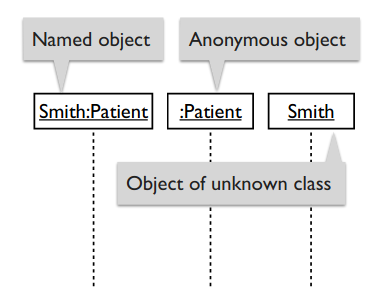
\includegraphics[width=0.45\textwidth]{obrazky-figures/names}
\end{minipage}


syntax jazyka PNTalk vytvára novú inštanciu následovne:

var := classname new.

kde var je dočasná premenná alebo miesto a classname je meno triedy. Problém je zjavný a to, že chýba akákoľvek informácia o mene inštancie. To nám hneď vylúči tretiu možnosť, pretože meno triedy je vždy známe. Varianty sú teda dve a to buď poskladať meno inštancie pomocou známych veličín ako názov miesta, meno triedy, krok simulácie či vygenerovať identifikačné číslo. Druhá varianta je uspokojiť sa s vedomím, že budú vznikať len Anonymné objekty bez názvu inštancie.

\subsection*{Čiara života}
Čiara života alebo inak lifeline je vertikálna čiara reprezentujúca život objektu začína pre každý objekt v dobe vytvorenia a končí deštrukciou objektu, alebo na konci simulácie. Jej vytvorenie je triviálne pokiaľ dokážeme určiť čas vytvorenia a zániku objektu. TODO ref

Je prekrytá bielym obdĺžnikom po dobu, kedy sa metóda objektu nachádza na zásobníku.

\subsubsection*{Na zásobníku}
Doba simulácie po ktorú sa prevádza metóda objektu je viazaná s volaním metód cudzích objektov a preto je nutno archivovať prechody a inštancie, ktoré ich vlastnia. Na tieto prechody potom namapovať prevádzané inštrukcie v chronologickom poradí.

\subsection*{Správa}
Správa vyžaduje poznať odosielateľa, príjemcu a hlavne o aký typ správy sa jedná. Poznáme tri typy:

Synchrónna
Asynchrónna
Odpoveď

zo syntaxe volania metódy pre cudzí objekt evidentne dokážeme zo simulácie odvodiť odosielateľa aj príjemcu.

var methodname: params

kde var je premenná s premennou nesúcou informáciu o mieste s objektom príjemcu. methodname je názov volanej metódy triedy príjemcu. params sú parametre metódy.

odosielateľ je inštancia, ktorá túto akciu zapríčinila svojim prechodom.

Ak metóda vracia hodnotu v simulácii je archivovaná ako odpoveď na správu nesúca údaje o správe na ktorú odpovedá a celú odpoveď.

TODO: Sync vs Async

\subsection*{Cyklus}

K odstráneniu redundantných scenárov značne pomôže zapúzdrenie cyklov, vždy hľadáme v prechodoch najmenší možný ohraničený celok, ktorý sa za sebou sekvenčne niekoľko krát opakuje.

\subsection*{Referovanie a prepájanie diagramov}
Podobne ako pri cykle hľadáme rovnaké, či podobné ohraničené sekvencie prechodov opakujúce sa v simulácii.

\section{Out-source simulácie}

Pre simuláciu bude generátor využívať jeden zo simulátorov objektovo orientovaných petriho sietí z variant bližšie špecifikovaných v kapitole :TODO: . Ako najschodnejšia varianta je zvolený pre túto prácu :TODO: . Aby sme si neuzavreli definitívne dvere k iným implementáciám simulátoru jazyka PNTalk je príhodné zamyslieť sa nad napojením generátoru na simulátor. 

\begin{enumerate}
	\item Varianta pridania kódovej časti do generátoru zjavne možná nie je z dôvodu rôznych implementačných jazykov. Voľba kotlinu ako implementačného jazyka je odôvodnená v sekcii :TODO: .
	
	\item Ponúka sa možnosť vytvoriť dynamickú knižnicu a volať funkcie simulátora z nej. Určite je táto možnosť schodné riešenie, ikeď tu doplácame na neschopnosť preložiť simulátor na všetkých platformách.
	
	\begin{note}
		Linuxová dynamická knižnica *.so nie je ekvivalentná s windowsovou *.dll
	\end{note}
	
	\item Veľmi podobné riešenie je spustiť binárny kód simulátoru s argumentami cestou ku kódu v jazyku PNTalk a zachytením výstupu cout. Oproti predchádzajúcej varianty, vyžaduje omnoho menej úprav.
	
	\item Posledná a taktiež zvolená varianta je pojať generátor ako distribuovaný systém :TODO: , ktorý bude k simulácii využívať komponentu simulátora s ktorou bude komunikovať vopred známym protokolom. To, že si komponenta simulátoru zavolá ďaľšiu komponentu prekladača do medzikódu nebude zo strany generátoru viditeľné. Dôležitý je len pevne daný protokol medzi generátorom a simulátorom, pretože nám to dáva možnosť implementácie simulátoru jednoducho meniť. Stačí aby dodržovali stanovené rozhranie.
	
\end{enumerate}

Distribuovaný systém môže nadobnúť odlišné fyzické formy, či už ide o skupinu osobných počítačov, prepojených lokálnou sieťou, skupinu pracovných staníc zdieľajúcích nielen súborové a databázové systémy, ale navyše aj zdieľaním výpočetnej sily procesora.\cite{}

Distribuovaný systém obsahujúci sadu procesov, ktoré medzi sebou udržujú formu komunikáciu. Okrem konkurenčného behu procesov, niektoré z procesov distribuovaného systému môžu prestať pracovať, pre príklad spadnúť alebo stratiť konektivitu, zatiaľ čo ostatné zostanú bežať a pokračovať v operácii. Toto je podstata čiastočných zlyhaní charakteristických pre distribuované systémy.

\section{Uživateľské rozhranie}

Pri návrhu grafického uživateľského rozhrania je dobré začať položením si otázky "Čo chceme zobrazovať?". Menej je však niekedy viac, pri príliš zložitom rozložení totiž strácame prehľadnosť. \\

\begin{enumerate}
	\item \textbf{Chceme zobraziť momentálne otvorený projekt} \\
	Reprezentáciou by mohol byť hierarchický strom, ktorý by mal v listoch uložené mená súborov a v uzloch mená adresárov. Listy, teda súbory, by mali vizuálnym effektom upozorniť ak je v súbore neuložená zmena. \\
	
	\begin{figure}[H]
		\centering
		\begin{minipage}{.4\textwidth}
			\centering
			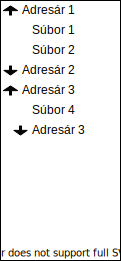
\includegraphics[scale=0.75]{obrazky-figures/UI-project-pane}
			\caption{ Projektový pohľad so schovaným uzlom ``Adresár 2'' a ``Adresár 4''}s
		\end{minipage}
		\begin{minipage}{.05\textheight} %spacer
			\quad
		\end{minipage}
		\begin{minipage}{.4\textwidth}
			\centering
			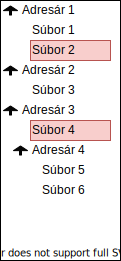
\includegraphics[scale=0.75]{obrazky-figures/UI-project-pane-dirty}
			\caption{Indikácia neuložených zmien v súboroch viditeľná na rozhraní.}
		\end{minipage}
	\end{figure}
	
	\item \textbf{Chceme zobraziť momentálne otvorený súbor s kódom} \\
	Realizujeme to ako editor zdrojového kódu s automatickým zvýrazňovaním kľúčových slov syntaxe jazyka PNTalk a mien z validných definícií. Potrebujeme zobrazovať čísla riadkov.
	\item \textbf{Chceme zobrazovať vygenerovaný diagram} \\
	Potrebujeme na to minimálne rovanko veľa miesta ako na editor zdrojového kódu. Pozadie by malo byť kontrastné vôči diagramu. Celá časť musí byť interaktívna, jednak kvôli pohybu a približovaniu diagramu v okne. Diagram by mal slúžiť ako nástroj na ladenie kódu. To znamená, že kliknutia na jednotlivé časti sekvenčného diagramu by mali vyznačiť reprezentáciu v kóde. Označenie správ by zasa malo zobraziť zmenu miest OOPN, ktoré prechody vyvolali. Označenie, ktoréhokoľvek miesta na čiare života by malo ukázať aktuálne hodnoty v miestach danej inštancie.
	\item \textbf{Chceme zobrazovať posledných \textit{x} riadkov logov}
	Je fajn dať uživateľovi vedieť čo sa deje formou správ, či už chybových alebo informačných. Správy sa musia dať kopírovať a musia byť viditeľné od najnovšej po najstaršiu.
	\item \textbf{Chceme zbytok funkcionalít ukryť do hornej lišty}
	V hornej lište by mali byť kategoricky roztriedené funkcie, s klávesovými skratkami u tých, u ktorých to dáva zmysel.
\end{enumerate}

\subsection{Rozloženie uživateľského rozhrania}

Nie je treba znovu vynaliezať koleso. Pri návrhu rozloženia elementov uživateľského rozhrania sa preto budeme inšpirovať úspešnými vývojovými prostrediami (Visual Studio, IntelliJ IDEA).
To samozrejme neplatí o netradičnom elemente vykresľujúci sekvenčný diagram, je to časť ktorá zobrazuje výstup a zároveň je to aj interaktívny debugger. Inšpiráciu pre tento element by sme hľadali márne, v bežných vývojových prostrediach sa nič podobné nenachádza.
Ničmenej je rovnako, ak nie viac, dôležitý ako editor zdrojového kódu, preto dostane rovnako veľké miesto. \\

Po zvážení veškerých nárokov na uživateľské rohranie vyšlo z procesu návrhu rozloženie na obr. :TODO:

\begin{figure}[H]
	\label{fig:ui-layout}
	\centering
	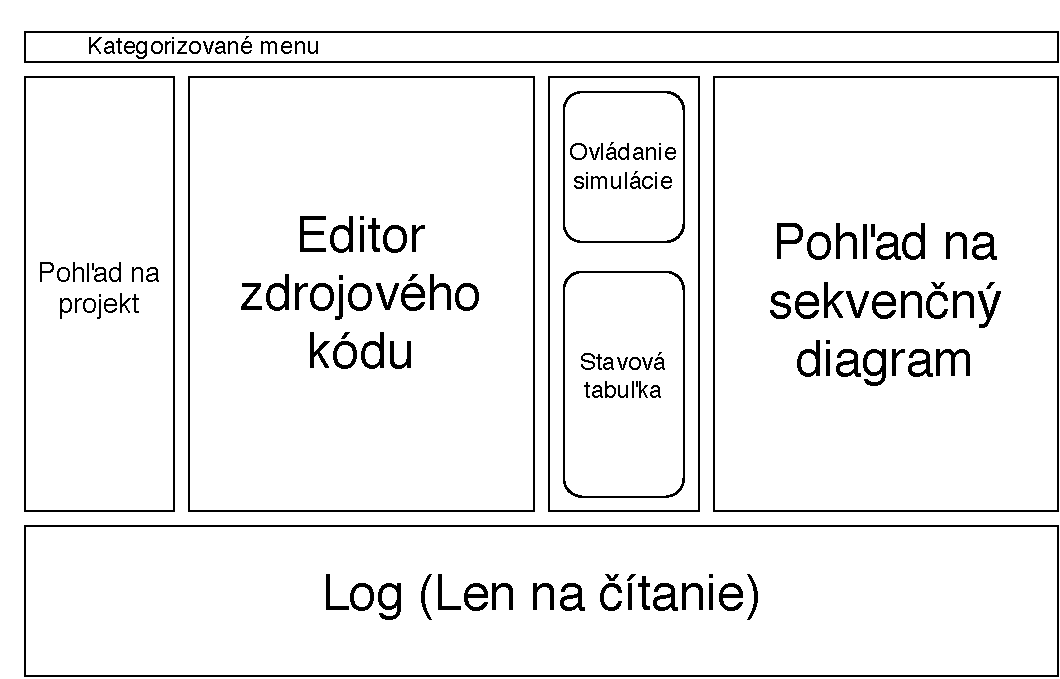
\includegraphics[scale=0.75]{obrazky-figures/UI-layout}
	\caption{Návrh rozloženia grafického uživateľského rozhrania}
\end{figure}



\chapter{Implementácia nástroja}

Implementoval som prácu v jazyku kotlin a prácu na ktorú som nadväzoval som upravil v jazyku C++, na ich prepojenie som využil verejne dostupné knižnice gRPC pre kotlin /cite{}https://github.com/grpc/grpc-kotlin a pre C++ \cite{}https://github.com/grpc/grpc. Prispôsobil som implementáciu simulátoru a prekladača medzikódu pre použitie s technológiou Docker a vytvoril spustiteľné obrazy týchto dvoch komponent skrz kontajnery dockeru dostupné na :TODO:. Na grafické uživatľské rozhranie bol použitý aplikačný rámec TornadoFX nad knižnicou JavaFX.

\section{Výber implementačného jazyka}

Práca nadväzuje na simulátor napísaný v jazyku C++, čo robilo z jazyka C++ prirodzenú voľbu pre hľadké naviazanie a kompatibilitu. Ničmenej ďaľším požiadavkom práce, akožto zadaním z oblasti blízkej jazyku PNTalk, bola motivácia držať implementačné jazyky týchto nástrojov blízko. :TODO: príklady Keďže väčšina prác beží na Jave a je do budúcna zmýšlaná ich kooperácia, získali sme ďaľší faktor ovplyvňujúci výber a to držať implementáciu blízko JVM (Java Virtual Machine). Od napojenia na simulátor priamo sa upustilo a zvolila sa varianta umožňujúca napojenie aj iných simulátorov napísaných v rôznych jazykoch. :TODO: Pre prácu bol zvolený ako implementačný jazyk Kotlin, zohľadňujúc požiadavky zmienené vyššie. Prispel k tomu rozvoj modernej doby a popularita akej sa teší Kotlin dnes. V roku 2017 ho Google učinil oficiálnym jazykom pre Android. \cite{tornadofx} Na platforme Github, ktorá hosťuje viac ako 100 miliónov repozitárov rôznych zdrojových kódov napísaných v rôznych jazykoch, bol Kotlin za rok 2019 štvrtý najrýchlejšie rastúci programovací jazyk s nárastom o 182\% oproti minulému roku. \cite{githuboctoverse}
V prvej polovici roku 2020, teda súčastnosti písania tejto práce, je celkovo na 15. priečke v obľúbenosti \cite{githubstats}.
%\vspace{1cm}

\begin{figure} [H]
	\label{chart:githubuse}
	\centering
	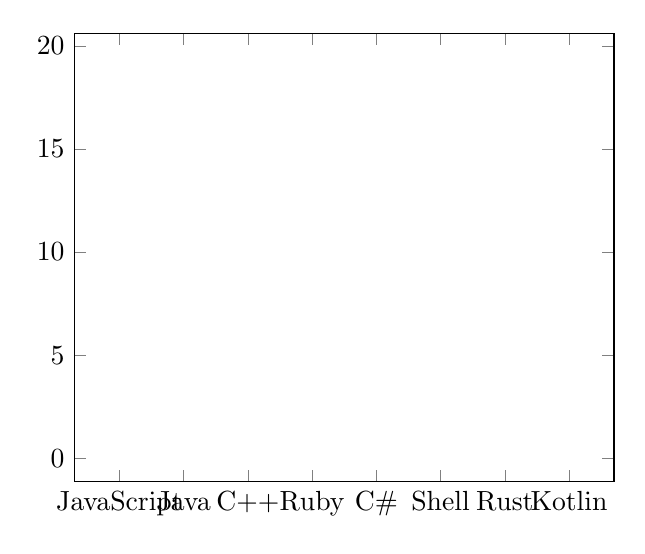
\begin{tikzpicture}
	\begin{axis}[
	%ybar=-1cm,
	%axis x line*=bottom,
	%axis y line*=left,
	%height=8cm, width=\textwidth,
	%bar width=0.8cm,
	%ylabel={Pridaný kód [\%]},
	symbolic x coords={JavaScript, Python, Java, Go, C++, TypeScript, Ruby, PHP, C\#, C, Shell, Scala, Rust, Swift, Kotlin},
	%x tick label style={rotate=45, anchor=east, align=left},
	%nodes near coords,
	%nodes near coords align={vertical},    
	]
	\addplot[gray,fill] coordinates {(JavaScript,18.789)};
	\addplot[gray,fill] coordinates {(Python,16.108)};
	\addplot[gray,fill] coordinates {(Java,10.731)};
	\addplot[gray,fill] coordinates {(Go,8.922)};
	\addplot[gray,fill] coordinates {(C++,7.636)};
	\addplot[gray,fill] coordinates {(TypeScript,7.334)};
	\addplot[gray,fill] coordinates {(Ruby,6.492)};
	\addplot[gray,fill] coordinates {(PHP,5.198)};
	\addplot[gray,fill] coordinates {(C\#,3.797)};
	\addplot[gray,fill] coordinates {(C,3.320)};
	\addplot[gray,fill] coordinates {(Shell,2.011)};
	\addplot[gray,fill] coordinates {(Scala,1.724)};
	\addplot[gray,fill] coordinates {(Rust,1.113)};
	\addplot[gray,fill] coordinates {(Swift,0.744)};
	\addplot[blue,fill] coordinates {(Kotlin,0.670)};
	\end{axis}
	\end{tikzpicture} 
	\caption{Pridaný kód za rok 2020, second quarter - stats report z github.com \cite{githuboctoverse}}
\end{figure}

\begin{figure} [H]
	\label{chart:githubgrow}
	\centering
\begin{tikzpicture}
\begin{axis}[
%ybar=-1cm,
%axis x line*=bottom,
%axis y line*=left,
%height=8cm, width=\textwidth,
%bar width=1cm,
%ylabel={Nárast [\%]},
symbolic x coords={Dart,Rust,HCL,Kotlin,TypeScript,PowerShell,Apex,Python},
%x tick label style={rotate=45, anchor=east, align=left},
%nodes near coords,
%nodes near coords align={vertical}        
]
\addplot[gray,fill] coordinates {(Dart,532)};
\addplot[gray,fill] coordinates {(Rust,235)};
\addplot[gray,fill] coordinates {(HCL,213)};
\addplot[blue,fill] coordinates {(Kotlin,182)};
\addplot[gray,fill] coordinates {(TypeScript,161)};
\addplot[gray,fill] coordinates {(PowerShell,154)};
\addplot[gray,fill] coordinates {(Apex,154)};
\addplot[gray,fill] coordinates {(Python,151)};           
\end{axis}
\end{tikzpicture} 
\caption{Najrýchlejšie rastúce jazyky - Octoverse report 2019 z github.com \cite{githuboctoverse}}
\end{figure}

\section{Implementácie distribuovaného systému}
Ako bolo zmienené v návrhu, generátor sa nebude viazať na simulátor ani prekladač do medzikódu. Namiesto toho budú prepojené v distribuovanom heterogénnom systéme.

\subsection{virtualizácia}

\subsubsection{Docker}
Bol zvolený prístup kontajnerov technológie Docker namiesto robustných virtuálnych strojov. Keďže virtuálne stroje obsahujú separátne jadro operačného systému ich veľkosť sa pohybuje okolo sto či tisíc Megabytov. Zatiaľ čo novo vzniknutý kontajner obsahuje len referenciu na obraz vrstvy súborového systému a nejaké meta dáta konfigurácie, čo vyjde na zopár desiatok kilobytov. \cite{kane2018docker} Vďaka tejto redukovanej pamäťovej stope sa urýchlil vývoj. Kontajnery sa spúšťali rýchlo, ani ich reštart nebol nijak časovo bolestivý.

\subsubsection{Nástroj Compose}

Docker Commpose je nástroj pre definovanie a beh multi-kontajnerových Docker aplikácií. S nástrojom sa používa súbor na konfiguráciu služieb aplikácie. Potom jediným príkazom dokážeme vytvoriť a spustiť všetky služby z konfigurácie. \cite{docker_docs}

\begin{lstlisting}[language=C++]
docker-compose up
\end{lstlisting}

Konfiguráciu bolo nutné vytvoriť pre službu simulátora a pre prekladač do medzikódu podľa :TODO: . Pre službu simulátora sa definoval port 51898 a pre prekladač do medzikódu port 51899. V konfigurácii na Obr. \ref{fig:docker-compose} vidíme otvorené práve tieto dva porty. Služby využívajú Docker obrazy so zdrojovými kódmi a prerekvizitami k prekladu. Sledovanie spusteného kontajneru je vyobrazené na Obr. \ref{fig:docker-desktop1}

\begin{figure}[H]
	\centering
\begin{lstlisting}[language=C++]
services:
simulator:
build: ./VM
ports:
- "51898:51898"
links: 
- "translator"
volumes: 
- "./VM:/VM:rw"
translator:
build: ./Translator
ports:
- "51899:51899"
volumes:
- "./Translator:/Translator:rw"
\end{lstlisting}
\caption{Použitá konfigurácia v docker-compose.yml}
\label{fig:docker-compose}
\end{figure}

\begin{figure}[H]
	\centering
	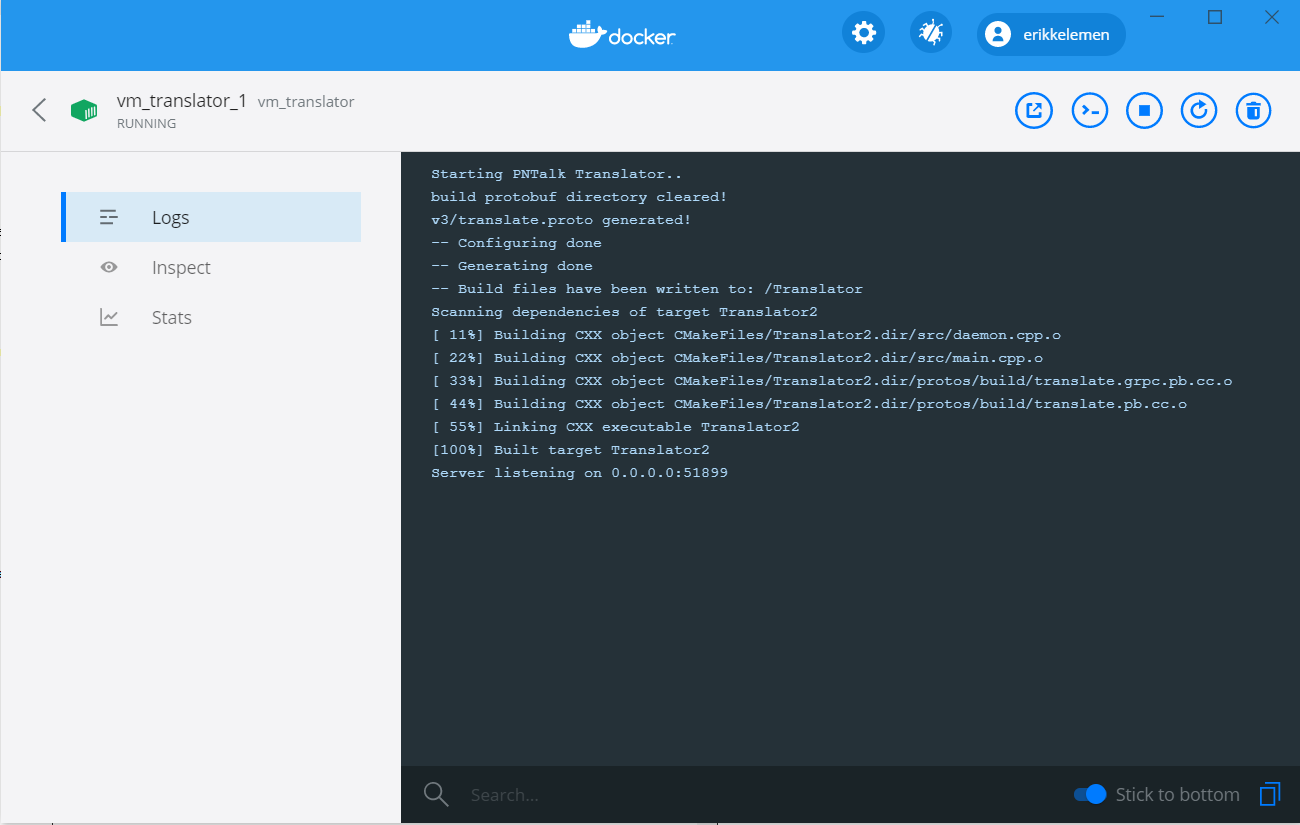
\includegraphics[scale=0.5]{obrazky-figures/PC-docker-desktop1}
	\caption{Náhľad do kontajneru v aplikácii Docker Desktop.}
	\label{fig:docker-desktop1}
\end{figure}




Kvôli prenositeľnosti komponent sa zvolil prístup kontajnerov namiesto robustných virtuálnych strojov. Keďže virtuálne stroje obsahujú separátne jadro operačného systému ich veľkosť sa pohybuje okolo sto či tisíc Megabytov. Zatiaľ čo novo vzniknutý kontajner obsahuje len referenciu na obraz vrstvy súborového systému a nejaké meta dáta konfigurácie, čo vyjde na zopár desiatok kilobytov. \cite{kane2018docker}
\subsubsection{HyperV}

\subsubsection{Nástroj Compose}

Commpose je nástroj pre definovanie a beh multi-kontajnerových Docker aplikácií. S nástrojom Compose sa používa YAML súbor na konfiguráciu služieb aplikácie. Potom jediným príkazom dokážeme vytvoriť a spustiť všetky služby z konfigurácie. \cite{docker_docs}

\subsection{Vzdialené volanie procedúr}

\subsubsection{gRPC}
gRPC je technológia navrhnutá pre vzdialenú medziprocesovú komunikáciu, tak aby prekonala nedostatky konvenčných technológií vzdialených volaní procedúr. Kde ostatné technológie používajú textový formát na prenos dát ako JSON alebo XML, gRPC využíva binárneho formátu. Protokol využíva HTTP/2 \cite{kuruppu2019grpc}, čo ho robí ešte rýchlejší vo vzdialenej medziprocesovej komunikácií.

\begin{lstlisting}[language=C++]
service Simulator {
	rpc simulate (SimulateRequest) returns (SimulateReply) {}
}

message SimulateRequest {
	string code = 1;
	string scenario = 2;
	int64 steps = 3;
}

message SimulateReply {
	int64 status = 1;
	string result = 2;
}
\end{lstlisting}

\section{Uživateľské rozhranie}

Implementácia vychádza z dobre pripraveného návrhu v sekcii :TODO: , ktorá bola realizovaná za pomoci kotlinovského aplikačného rámcu TornadoFX nad softvérovou platformou JavaFX.

\subsection{Bohaté internetové aplikácie}

Bohaté internetové aplikácie, (Rich Internet Aplication), niekedy tiež v literatúre pod názvom moderné internetové aplikácie, /cite{psatweb} sú webové aplikácie poskytujúce responzivitu a sú "bohaté" v zmysle funkcionality a možností desktopových aplikácií. Ranné internetové aplikácie poskytovali len HTML grafické uživateľské rozhranie, ktoré dokázalo poslúžiť jednoduchým cieľom, no nemalo ani vzhľad ani responsivitu RIA hlavne kvôli pomalému internetovému spojeniu. RIA je teda výsledkom dnešnej doby poskytujucej vyššiu responzivitu a pokročilejšie grafické uživateľské rozhrania.
\cite{deitel2008ajax}

Na tvorbu bohatých internetových aplikácií, môžme využiť celú radu aplikačných rámcov, tu vudú spomenuté len varianty zvažované pre túto prácu.

\subsubsection{Ajax}

Výraz Ajax (Asynchronous JavaScript and XML) vznikol vo februáry roku 2005 od Jamesa Garretta. Ajax aplikácie dovoľujú čiastočné aktualizácie stránky. To znamená aktualizovať individuálne časti webu bez nutnosti obnoviť celú stránku. To vytvára viac responzívne GUI ako predtým, dovoľujúci uživateľom ďalej pracovať so stránkov, zatiaľ čo server zpracováva požiadavky. \\

Technológie stojace za Ajaxom - XHTML, CSS, JavaScript, the DOM, XML a XMLHttpRequestobject — nie sú nové. Vlastne už v 90 rokoch existujú príklady asynchrónnych aktualizácií stránky, ktoré rozultovali v JavaScript \cite{deitel2008ajax}. Ničmenej popularita Ajaxu dramaticky narástla až po jeho pomenovaní v roku 2005. \\

Ajax sa ukázal ako nevhodný pre prácu, kvôli nízkej abstrakcii.

\subsubsection{Flex}

\subsubsection{JavaFX}
 JavaFX je softvérová technológia na vytváranie bohatých internetových aplikácií (Rich Internet Application) s obsahom cez širokú škálu platforiem a zariadení.
Táto technológia bola zvolená k implementácii uživateľského rozhrania. Jazyk sa pôvodne nazýval F3 (Form Follows Function) a jeho priekopníkom a tvorcom bol Chris Oliver, ktorý v tej dobe pracoval pre firmu SeeBeyond \cite{dea2011javafx}. Meno bolo zmenené v roku 2007 na JavaFX. \cite{anderson2009essential}

The first version of JavaFX Script was an interpreted language, and was considered a prototype of the compiled JavaFX Script language that was to come later

Najprv vznikol JavaFX Script ako interpretovaný jazyk, ktorý bol považovaný za prototyp :TODO: kompilovaného JavaFX Script jazyka, ktorý ho mal nahradiť. Tento deklaratívny skriptovací jazyk, tiež staticky typovaný ako Java využíval knižnice Javy a dokonca mohol volať jej metódy, či inštancovať jej triedy. \cite{weaver2007javafx}

V roku 2011 verzia JavaFX 2.0 prestala využívať JavaFX Script a vymenila ho za Javu a JavaFX 2.0 API. \cite{dea2011javafx}Jeho hlavnou nevýhodou bola prerekvizita Javy, ktorá ho ako jediná vedela preložiť. Týmto krokom sa technológia JavaFX dostala k jazykom bežiacim na JVM ako Groovy, JRuby či Kotlin.

\subsubsection{TornadoFX}

Jedna z hlavných výhod pre kotlin spomenutá v sekcii :TODO: bola
jeho 100 \% interoperabilita s existujúcimi Java knižnicami, vrátane JavaFX. I keď kotlin môže využívať JavaFX priamo rovnakým spôsobom ako v Jave, niektorí verili, že Kotlin má jazykové predispozície aby mohol usmerniť a zjednodušiť vývoj JavaFX aplikácií. Eugen Kiss prototypoval vrstvu nad JavaFX ako KotlinFX, jeho nápad neskôr priviedol ku zdarnejšiemu koncu Edvin Syse v januáry 2016\cite{tornadofx}, keď vydal TornadoFX.
\\
TornadoFX usiluje o to, aby znateľným spôsobom minimalizovalo rozsah potrebného kódu na napísanie JavaFX aplikáce. Zahŕňa typovú kontrolu nad komponentmi pri skladaní komponent uživateľského rozhrania a prináša rozšírenia kotlinu ako delegované vlastnosti a injekcia závislostí. TornadoFX je ukážkový príklad ako Kotlin dokáže zúsporniť kód napísaný v Jave.

\subsection{Editor Zdrojového kódu}

V sekcii \ref{sec:TR-code-editor} boli vymenované niektoré funkcionality, ktoré nesmú chýbať v moderných editoroch zdrojového kódu. Z nich bolo implementované zvýrazňovanie kľúčových slov jazyka PNtalk a zvýrazňovanie všetkých validne definovaných názvov tried, prechodov, miest, synchrónnych portov a metód.

Zvýrazňovanie zaisťuje asynchrónna funkcia computeHighlighting volaná nad textom z editoru. Je postavená na vyhľadávaní regulárnych výrazov. Globálne v celom rámci sa zvýrazňujú kľúčové slová jazyka PNTalk a mená tried. V rámci danej triedy sa k nim pridá vyhľadávanie názvov prechodov, miest, synchrónnych portov definovaných však len v rozsahu danej triedy.

\subsection{Projektový pohľad}

\subsection{Diagram ako výstup aj interaktívny ladiaci nástroj}

\chapter{Testovanie}

\chapter{Záver}

Cieľom práce bolo implementovať nástroj pre generovanie sekvenčných diagramov. Zámer práce sa podarilo splniť vo všetkých bodoch.

V práci ma prekvapilo, že som sa dostal k distribuovanému systému, čo som pôvodne od zadania neočakával. Viac komponent pracujúcich na spoločnej úlohe bol koncept, ktorý som si chcel už dlhší čas vyskúšať. Preto sa jednalo o prekvapenie značne príjemné. Dovolilo mi to pochopiť výhody mikroservís z viac praktického hľadiska. \\

V práci by som chcel pokračovať implementovaním filtrovania správ a hľadaním v dátach simulácie vzory cyklov či podmienok. Potenciál vidím aj v zlepšení simulátoru, ktorý by mohol dosahovať lepších časov simulácie a dať tak možnosť vykreslovať sekvenčný diagram responzívne, prakticky ihneď po akejkoľvek zmene v kóde jazyka PNTalk. Za úvahu by stálo i rozšírenie vývojového prostredia.
Editor kódu zvláda v terajšom stave zvýrazňovanie v kóde a mapovanie častí sekvenčného diagramu k odpovedajúcim častiam kódu, ktoré popisujú chovanie danej časti. Obe tieto funkcionality náramne uľahčujú tvorenie a ladenie kódu, ale editor stále postráda niektoré vlastnosti inteligentnejších vývojových prostredí. Editor kódu by mohol skúšať dopĺňať kód podľa prvých napísaných znakov a pozícií v kóde. Implementované by to mohlo byť rozhodovacím stromom. 

Práca demonštroje automatický prevod objektovo orientovaných Petriho sietí na sekvenčné diagramy, generovanie však pokrýva len podmnožinu sekvenčných diagramov. Objekty Actors vystupujúce v konvenčne vytvorených sekvenčných diagramoch sú v práci zanedbané (keďže informáciu na rozlíšenie obyčajných objektov od Actors nedokázali poskytnúť definície v kóde, ani následná simulácia) a Actors preto vystupujú len ako všeobecné objekty. Ďaľší zrejmý nedostatok vyplýva z naviazania na neúplnú implementáciu simulátora, ktorá neumožňuje simuláciu všetkých validných konštrukcií jazyka PNTalk, len ich podmnožinu. Istou kompenzáciou jest architektúra navrhnutá ako distrubovaný systém, ktorá robí tento problém ľahko riešiteľným v budúcnosti po implementovaní vhodnejšej varianty simulátora. Na Záver je vhodné položiť si otázku či sme boli úspešný.
To nám zodpovie sada validačných testov. Jedná sa o netriviálne Petriho siete zadefinované v jazyku PNTalk, ktorých vygenerované výstupy boli porovnané s tými ručne vytvorenýmí. Okrem validity vzišla motivácia zaznamenať výsledky aj časovej náročnosti. Časová náročnosť sa merala pre samotný proces generácie sekvenčných diagramov ako aj celkovo beh v spolupráci externých komponent. Plán bol vytýčiť hranice, pre ktoré by bolo reálne simulovať a vykreslovať výsledok generácie ihneď pri zmene vstupnęho kódu. Kvôli neuspokojivým výsledkom v tomto teste (:TODO: graf) sa z pokusu o implementácie funkcie "hot-reload" upustilo. 





 

